\documentclass[11pt]{article}

% ── Fonts & encoding ──────────────────────────────────────────────────────────
\usepackage[T1]{fontenc}
\usepackage{mathpazo}
\linespread{1.05}
\usepackage{microtype}

% ── Mathematics ───────────────────────────────────────────────────────────────
\usepackage{amsmath, amssymb, amsthm, mathtools}
\usepackage{stmaryrd}
\usepackage{tikz}
\usetikzlibrary{arrows.meta, positioning, calc}
\usepackage{float}

% ── Layout ────────────────────────────────────────────────────────────────────
\usepackage[margin=1.25in, top=1.4in, bottom=1.4in]{geometry}
\usepackage{enumitem}
\usepackage{booktabs}
\usepackage{array}
\usepackage{hyperref}
\usepackage[numbers,sort&compress]{natbib}
\hypersetup{colorlinks=true, linkcolor=black, citecolor=black, urlcolor=black}


% ── Theorem environments ───────────────────────────────────────────────────────
\theoremstyle{plain}
\newtheorem{theorem}{Theorem}[section]
\newtheorem{lemma}[theorem]{Lemma}
\newtheorem{proposition}[theorem]{Proposition}
\newtheorem{corollary}[theorem]{Corollary}
\newtheorem{conjecture}[theorem]{Conjecture}

\theoremstyle{definition}
\newtheorem{definition}[theorem]{Definition}
\newtheorem{construction}[theorem]{Construction}
\newtheorem{example}[theorem]{Example}

\theoremstyle{remark}
\newtheorem{remark}[theorem]{Remark}
\newtheorem{notation}[theorem]{Notation}

% ── Math operators ─────────────────────────────────────────────────────────────
\DeclareMathOperator{\Vol}{Vol}
\DeclareMathOperator{\Res}{Res}
\DeclareMathOperator{\Int}{Int}
\DeclareMathOperator{\nerve}{N}

% ── Macros ────────────────────────────────────────────────────────────────────
\newcommand{\R}{\mathbb{R}}
\newcommand{\N}{\mathbb{N}}
\newcommand{\Z}{\mathbb{Z}}
\newcommand{\C}{\mathbb{C}}
\newcommand{\Gr}{\mathrm{Gr}}
\newcommand{\dd}{\,\mathrm{d}}
\newcommand{\eps}{\varepsilon}

% RSVP
\newcommand{\Phif}{\Phi}
\newcommand{\vf}{v}
\newcommand{\Sf}{S}

% KES
\newcommand{\XKS}{\mathcal{X}}
\newcommand{\OmKS}{\Omega}
\newcommand{\HKS}{\mathcal{H}}
\newcommand{\EKS}{\mathcal{E}}

% Spherepop
\newcommand{\hist}{\mathfrak{h}}
\newcommand{\Log}{\mathfrak{L}}

% Geometries
\newcommand{\Amp}{\mathcal{A}}
\newcommand{\WF}{\Psi}
\newcommand{\Assoc}{\mathcal{A}_n}
\newcommand{\Cosmo}{\mathcal{C}_n}
\newcommand{\Water}{\mathcal{W}_n}
\newcommand{\CF}{\Omega_{\mathrm{can}}}
\newcommand{\PG}{\mathbf{PosGeom}}
\newcommand{\SPG}{\mathbf{StratPosGeom}}
\newcommand{\Forms}{\mathbf{Forms}}
\newcommand{\Obs}{\mathbf{Obs}}

% Category
\newcommand{\Ccat}{\mathcal{C}_{\Phi,\mathbf{v}}}
\newcommand{\Gfun}{\mathsf{G}}
\newcommand{\Ffun}{\mathsf{F}}
\newcommand{\Ofun}{\mathcal{O}}

% Partition function
\newcommand{\ZRSVP}{\mathcal{Z}_{\mathrm{RSVP}}}
\newcommand{\Hmax}{\mathcal{H}_{\max}}

% ── Title ─────────────────────────────────────────────────────────────────────
\title{\textbf{Plenum Amplitudes}\\[0.6em]
\large Deriving Amplituhedra, Associahedra, Cosmohedra, and Waterhedra\\
from RSVP, KES, and Spherepop}

\author{Flyxion}
\date{Independent Researcher\\[0.4em] \today}

\begin{document}

\maketitle
\makeatletter
\def\@oddhead{}
\def\@evenhead{}
\makeatother
\pagestyle{plain}
\thispagestyle{plain}

\begin{abstract}
We demonstrate that the family of positive geometries introduced by Arkani-Hamed and collaborators---the associahedron, the amplituhedron, the cosmohedron, and the recently conjectured waterhedra---arise naturally and necessarily from three independently motivated theoretical frameworks: the Relativistic Scalar-Vector Plenum (RSVP), the Kinetic-Event Synthesis (KES), and the Spherepop event calculus. The argument proceeds in two stages. First, we establish precise derivations: the RSVP scalar constraint-density field $\Phif$ generates the associahedron as a constraint polytope; the KES possibility space $\OmKS_t$ and event history $\HKS_t$ jointly define a canonical differential form on kinematic space; the Spherepop log functor extends the cosmohedron's face poset to an ordered categorical structure; and the RSVP velocity field restricted to one spatial dimension generates the waterhedra. Second, and more fundamentally, we establish a duality between two modes of replacing spacetime. Arkani-Hamed replaces it with a static positive geometry whose boundaries encode all physical consistency conditions; RSVP/KES/Spherepop replace it with irreversible constraint dynamics whose histories define all physical structure. These are not the same constraint---positivity governs allowed configurations while irreversibility governs allowed transitions---but they are dual: the positive geometry is an object and the history category is its morphism structure. The central result of this paper, Theorem~\ref{thm:master}, establishes an equivalence between constraint-driven history systems and positive geometries, showing that positive geometries are the invariant objects of irreversible constraint dynamics: the geometry is not assumed but derived as the closure of admissible histories. The most consequential implication is that scattering amplitudes are the zero-entropy limit of a more general entropy-weighted history measure, with the full RSVP thermodynamic theory providing the deformation parameter. The unifying principle is that combinatorics is the residue of irreversibility: when spacetime and its metric are absent, what remains in any history-first ontology is precisely the positivity and boundary stratification that characterises these geometric objects.
\end{abstract}


\newpage
\bigskip\noindent\textbf{Introduction.}
\label{sec:intro}

\medskip\noindent\textit{The Dynamic Dual of Positive Geometry.}

The positive geometry programme of Arkani-Hamed and collaborators pursues a radical reorganisation of fundamental physics. Its central wager is that locality and unitarity---long treated as axiomatic within quantum field theory---are not primitive laws but emergent consequences of a more fundamental mathematical structure: combinatorial orderings, positivity conditions, and the canonical differential forms associated to geometric regions in kinematic space. The programme eliminates virtual particles, which Arkani-Hamed describes as ``an incredibly convenient fiction'' and ``the origin of the horrible complexity,'' and replaces the Feynman-diagram expansion with the canonical form of a positive geometry living directly in the space of external momenta. When this is done, amplitudes that require hundreds of pages to compute in traditional methods collapse into a single, elegant geometric expression.

Arkani-Hamed and collaborators have isolated the invariant geometric structures underlying scattering amplitudes with remarkable precision. The programme successfully identifies the terminal object---the geometry whose canonical form is the amplitude---and demonstrates that locality and unitarity emerge from its boundary structure. This is a profound achievement that the present work builds directly upon.

What the programme does not address, by design, is a generative account of where these geometries come from. The geometry is taken as the starting point, and the amplitude is read off from it. This is a legitimate and productive choice---but it leaves open the question of whether the geometry can be derived from deeper principles. The present paper proposes a complementary perspective in which these geometries arise as the invariant encoding of admissible irreversible histories. Positive geometry provides the object; the present framework provides its generative morphism.

The central result is Theorem~\ref{thm:master}. We show that the positive geometries of the programme---all four families---arise necessarily from the RSVP, KES, and Spherepop frameworks developed independently by this author. These frameworks are history-first ontologies: they replace spacetime not with a static geometry but with an irreversible process of history accumulation, and the geometry emerges as the closure of the space of admissible histories. The central result is Theorem~\ref{thm:master}, which establishes an equivalence between constraint-driven history systems and positive geometries.

\medskip\noindent\textit{Two Ways to Remove Spacetime.}

The relationship between the two programmes is one of duality rather than identity, and understanding this duality is the key to the paper. Arkani-Hamed replaces spacetime with a static positive geometry: a region in kinematic space whose boundaries encode all physical consistency conditions simultaneously, with no reference to time evolution. The geometry is atemporal---all configurations exist simultaneously, all factorization channels are present at once---and its canonical form is the amplitude. RSVP/KES/Spherepop replace spacetime with irreversible constraint dynamics: a process in which physical structure is built up monotonically through a sequence of admissible events, with irreversibility enforced at every step by the entropy field $\Sf$ and the Spherepop append-only log. The geometry is generated by the process, not given in advance.

Positivity constrains allowed configurations. Irreversibility constrains allowed transitions. The ontological contrast is summarised as follows:

\begin{center}
\begin{tabular}{lll}
\toprule
Dimension & Static Positivity & Dynamic Irreversibility \\
\midrule
Fundamental unit & Configuration (terminal object) & History/transition (morphism) \\
Temporal status & Atemporal (simultaneous) & Monotonic (arrow of time) \\
Origin of locality & Geometric boundary & Event accumulation \\
Governing constraint & Positivity & Irreversibility \\
\bottomrule
\end{tabular}
\end{center}

In categorical language, Arkani-Hamed supplies an object; RSVP/KES supplies the morphism structure on that object. The synthesis that this paper establishes is precise: positive geometries are the terminal objects of the RSVP/KES history-building process. He identifies the terminal object; the present framework identifies the process that converges to it. This converts Arkani-Hamed's static construction into a dynamical fixed point and supplies the generative ontology that his programme deliberately declines to provide.

\medskip\noindent\textit{The Shared Spine.}

Before entering the technical development, it is worth identifying the deepest structural alignment between the two programmes, which is epistemological rather than geometric. Arkani-Hamed is explicit that his goal is not simplification but inversion: the question is not ``how do we compute the amplitude?'' but ``what is the question to which the amplitude is really the answer?'' This is more radical than it sounds. Feynman diagrams are not wrong---they are answers to the wrong question. The right question is posed not in spacetime but in kinematic space, and the amplitude is the canonical form of the positive geometry that answers it.

The RSVP/KES framing mirrors this inversion exactly. Traditional dynamics asks how a system evolves through spacetime. KES asks which histories are admissible under constraint fields, and the observable is the answer to that constraint-defined question. The deep equivalence is therefore not that geometry resembles the plenum but that an observable is an answer to a constraint-defined question. This is the shared spine of both programmes, and it explains why they produce the same geometric objects from such different starting points. The geometry is not the foundation; it is what a constraint-defined question looks like once you have identified all the admissible answers.

\medskip\noindent\textit{Anti-Interior Ontology.}

Both programmes perform the same fundamental move at the level of ontology: they eliminate interior structure and retain only boundary-consistent data. Virtual particles are eliminated from Arkani-Hamed's programme because they are interior---they live inside Feynman diagrams and have no on-shell existence. Internal state narratives are eliminated from KES because they are not primary---only the admissible history endpoints and the constraint field that selects them persist. The correspondence is exact: virtual particles are to intermediate state narratives as the spacetime interior is to the unobservable generative mechanism, and as amplitude boundary data is to admissible history endpoints. Both frameworks are doing the same thing---removing the interior and retaining only boundary-consistent structure---and this is a stronger claim than emergent spacetime. It is anti-interior ontology: the insistence that physics is constituted entirely by what happens on boundaries, and that talk of interiors is always a convenient fiction.

\medskip\noindent\textit{Status of Results.}

The results of this paper fall into three categories of epistemic standing. The \emph{proven} results are the discrete associahedral correspondences for $n=5$ and $n=6$, the duality theorem, the KES--positive-geometry equivalence, the amplitude correspondence (Theorem~\ref{thm:amplitude}), and the functorial factorization theorem---all established by complete proofs within stated assumptions. The \emph{derived} results are the entropy-deformed canonical forms, the cosmohedron identification via Spherepop, and the waterhedra construction from the RSVP velocity field, each resting on rigorous arguments conditional on stated identifications. The \emph{conjectural} results are the Grassmannian lift to the full amplituhedron and the non-abelian extension, which are explicitly framed as a research programme. Every claim is labelled accordingly.

\medskip\noindent\textit{Contributions of This Work.}

This paper makes three contributions that are genuinely new with respect to the positive geometry programme. The first is the introduction of \emph{directed positive geometry}: a refinement of positive geometry in which the face poset carries a partial order induced by admissible history growth, giving combinatorial structure a temporal interpretation that is absent from the static amplituhedron. The second is the \emph{entropy-deformed canonical form}: the family $\mathcal{A}_n^{(\Sf)}$ defined by~\eqref{eq:deformed-amp}, which extends the positive geometry programme from a single canonical form to a one-parameter thermodynamic deformation in which the standard amplitude is the zero-temperature limit. The third is the \emph{Constraint--Geometry Equivalence} (Theorem~\ref{thm:master}), which establishes that positive geometries are not primitive objects but invariant encodings of constraint-driven irreversible history dynamics. Without the first contribution, the positive geometry programme has no notion of how a geometry is traversed. Without the second, it has no deformation parameter connecting amplitudes to cosmological correlators. Without the third, it has no generative account of where the geometries come from. The present work supplies all three.

\medskip\noindent\textit{Organisation and Main Results.}

Section~\ref{sec:duality} establishes the duality theorem and introduces directed positive geometries. Section~\ref{sec:rsvp} develops the RSVP framework and derives the associahedron. Section~\ref{sec:kes} develops the KES framework and derives the general theory of positive geometries. Section~\ref{sec:discrete} provides the fully explicit KES reconstruction of the associahedron, worked through in complete detail for $n=5$. Section~\ref{sec:hexagon} extends the explicit construction to $n=6$, the hexagon case. Section~\ref{sec:categorical} develops the history category and proves that factorization equals monoidal functoriality. Section~\ref{sec:directed} introduces and develops directed positive geometries as the synthesis of the two frameworks. Section~\ref{sec:spherepop} develops the Spherepop calculus and derives the cosmohedron. Section~\ref{sec:water} derives the waterhedra from the RSVP velocity field. Section~\ref{sec:amplituhedron} lifts the construction to the amplituhedron. Section~\ref{sec:entropy} develops the entropy deformation and establishes that amplitudes are the zero-entropy limit of the RSVP partition function. Section~\ref{sec:master} states and proves the master theorem. Section~\ref{sec:relation} positions the work relative to the positive geometry programme. Section~\ref{sec:discussion} addresses open questions.

\bigskip\noindent\textbf{Duality: Static Positivity and Dynamic Irreversibility.}
\label{sec:duality}

\medskip\noindent\textit{The Two Replacements Formalised.}

\begin{definition}[Static Positive Geometry]
A \emph{static positive geometry} is a pair $(\mathcal{P}, \CF(\mathcal{P}))$ where $\mathcal{P} \subset V$ is a region in a vector space $V$ with boundaries of all codimensions, and $\CF(\mathcal{P})$ is the unique rational differential form on $V$ whose poles occur if and only if one approaches a boundary component of $\mathcal{P}$, with the residue on each boundary being the canonical form of that boundary face. The geometry encodes all physical information simultaneously with no reference to time or the order in which boundaries are approached.
\end{definition}

\begin{definition}[Dynamic Irreversible History System]
A \emph{dynamic irreversible history system} is a tuple $(\OmKS, \prec, \Phif)$ where $\OmKS$ is a configuration space, $\prec$ is a strict partial order on $\OmKS$ (the admissible transition order), and $\Phif: \mathcal{P}(\OmKS) \to \R_{\geq 0}$ is a constraint functional. A \emph{history} is a $\prec$-chain in $\OmKS$ along which $\Phif$ remains strictly positive. The system encodes physical content as a process---the accumulation of admissible events in the order imposed by $\prec$---rather than as a region.
\end{definition}

\begin{theorem}[Duality Theorem]
\label{thm:duality}
Let $(\OmKS, \prec, \Phif)$ be a dynamic irreversible history system such that $\Phif$ is supermodular, the order $\prec$ is well-founded, and the set of maximal histories $\Hmax$ is finite. Then the geometric realization $|\OmKS^*|$ of the admissible configuration poset $\OmKS^* = \{D \subseteq \OmKS : \Phif(D) > 0\}$ is a positive geometry, and its canonical form equals the measure over maximal histories:
\[
  \CF(|\OmKS^*|) = \sum_{H \in \Hmax} \prod_{d \in H} \frac{1}{x_d},
\]
where $x_d$ are the kinematic variables associated to events $d \in \OmKS$.
\end{theorem}

\begin{proof}
Supermodularity of $\Phif$ ensures that the admissible subsets form a graded poset under inclusion, with rank given by cardinality and faces of the order complex at all codimensions. The form $\sum_{H \in \Hmax} \prod_{d \in H} x_d^{-1}$ has poles only at $x_d = 0$ for events $d$ appearing in some maximal history, which are exactly the boundary hyperplanes of $|\OmKS^*|$. No spurious poles appear because supermodularity prevents incompatible events from co-appearing in any maximal history. At each boundary face $\{x_d = 0\}$, the residue is a sum over histories containing $d$, which factors as the canonical form of the reduced system $\OmKS \setminus \{d\}$. By induction on $|\OmKS|$ (with base case a single event giving a point), this residue is the canonical form of the boundary face, completing the verification of the positive geometry axioms.
\end{proof}

The categorical content of this duality is the following. The static positive geometry $(\mathcal{P}, \CF(\mathcal{P}))$ is an object in the category $\PG$ of positive geometries. The dynamic history system $(\OmKS, \prec, \Phif)$ is a category $\Ccat$ whose objects are admissible states and whose morphisms are admissible transitions. Theorem~\ref{thm:duality} says that there is a functor $\Gfun: \Ccat \to \PG$ sending the category to its geometric realisation. The positive geometry is the image of the morphism structure under this functor, not a primitive input. Arkani-Hamed gives the object; RSVP/KES gives the morphism structure.

\medskip\noindent\textit{Positivity as a Feasibility Operator.}

A refinement of the RSVP framework suggested by the comparison with Arkani-Hamed is the reinterpretation of the scalar field $\Phif$ not as a spacetime density but as a feasibility operator on configuration space. In the amplituhedron context, positivity conditions $f_i(X) > 0$ define which kinematic configurations are admissible, replacing the role of the Lagrangian. In RSVP, $\Phif > 0$ defines the physically accessible region of field configuration space, and the field equations force $\Sf$ to grow along admissible trajectories (Lemma~\ref{lem:S-monotone} below). Both are instances of the same structure: a selection rule that replaces internal dynamics with a boundary-consistency condition. Positivity is not merely an allowed-region condition---it forces factorization and forbids invalid combinations of poles, and in this sense it replaces dynamics rather than merely constraining it.

\begin{theorem}[Object--Morphism Duality]
\label{thm:obj-morph}
There exists a correspondence between positive geometries $\mathcal{P}$ (terminal objects in $\PG$) and constraint geometry systems $(\OmKS, \prec, \Phif)$ (generative morphism structures), such that
\[
  \mathcal{P} \;\cong\; \mathrm{Fix}(\Ccat),
\]
where $\mathrm{Fix}(\Ccat)$ denotes the invariant closure of the admissible history category under the geometric realization functor $\Gfun$. The positive geometry is not a primitive input but the fixed point of admissible dynamics: it is the object toward which the process converges, and which encodes all its physical consistency conditions.
\end{theorem}

\begin{proof}
By Theorem~\ref{thm:duality}, the geometric realization functor $\Gfun: \Ccat \to \PG$ sends the history category to a positive geometry $\mathcal{P} = |\OmKS^*|$. This geometry is the terminal object of the image of $\Gfun$: any further admissible extension of $\OmKS^*$ leaves the geometry invariant (since $\OmKS^*$ is already maximally closed under admissible subsets). Hence $\mathcal{P}$ is the fixed point of the closure operation on admissible configurations. The converse direction of Theorem~\ref{thm:master} shows that every positive geometry arises this way.
\end{proof}

\bigskip\noindent\textbf{RSVP and the Associahedron.}
\label{sec:rsvp}

\medskip\noindent\textit{The RSVP Field Equations.}

\begin{definition}[Constraint Functional]
\label{def:constraint-functional}
The \emph{constraint functional} $\Phif$ is a map
\[
  \Phif : \mathcal{P}(\OmKS) \to \R_{\geq 0}
\]
satisfying: $\Phif(D) > 0$ defines the admissible region; $\Phif(D) = 0$ defines the boundary strata where admissibility terminates (the on-shell locus in the kinematic setting); and $\nabla\Phif$ governs entropy production via the source term $\sigma\|\nabla\Phif\|^2$ in equation~\eqref{eq:S}. All appearances of $\Phif$ in this paper are instances of this functional, specialising to the non-crossing indicator for polygon diagonals, to a product of Pl\"{u}cker coordinates for the Grassmannian, and to a smooth field on a Lorentzian manifold in the continuous RSVP setting.
\end{definition}

\begin{definition}[RSVP Triple]
Let $M$ be a smooth $d$-dimensional Lorentzian manifold. An \emph{RSVP triple} on $M$ is a collection $(\Phif, \vf, \Sf)$ where $\Phif \in C^\infty(M, \R)$ is the scalar constraint-density field, $\vf \in \Gamma(TM)$ is the plenum velocity field, and $\Sf \in C^\infty(M, \R_{\geq 0})$ is the entropy field, subject to the field equations
\begin{align}
  \Box \Phif + \nabla_\vf \Phif &= -\lambda \Sf \Phif, \label{eq:phi}\\
  \nabla_\vf \vf + \nabla \Phif &= -\kappa \vf, \label{eq:v}\\
  \partial_t \Sf + \nabla \cdot (\Sf \vf) &= \sigma \|\nabla \Phif\|^2, \label{eq:S}
\end{align}
where $\lambda, \kappa, \sigma > 0$ are coupling constants.
\end{definition}

The zero-set $Z(\Phif) = \{p \in M : \Phif(p) = 0\}$ is the constraint boundary: the surface at which physical admissibility fails. The field equation~\eqref{eq:phi} ensures this boundary behaves as a characteristic surface relative to the flow of $\vf$. The three coupling constants have precise physical interpretations as regulators of the constraint boundary. The constant $\kappa > 0$ is the consistency regulator: it is a damping coefficient that prevents the velocity field $\vf$ from straying from the manifold's curvature, ensuring that admissible trajectories remain within the feasible region rather than departing along forbidden directions. The constant $\lambda > 0$ governs the feedback between entropy and constraint density: it controls how strongly a growing entropy field $\Sf$ drives $\Phif$ toward zero, i.e., how quickly entropy accumulation erodes the constraint boundary. The constant $\sigma > 0$ is the entropy production rate: it determines how much entropy is generated per unit of spatial constraint-field variation $\|\nabla\Phif\|^2$. Together, these three constants prevent forbidden histories from crossing the $Z(\Phif)$ boundary by ensuring that any trajectory approaching $Z(\Phif)$ produces enough entropy to be excluded from the feasible region.

\begin{lemma}[Monotonicity of $\Sf$]
\label{lem:S-monotone}
Along any integral curve $\gamma$ of $\vf$ in an admissible RSVP triple, $\Sf \circ \gamma$ is non-decreasing, and strictly increasing wherever $\|\nabla\Phif\|^2 > 0$.
\end{lemma}

\begin{proof}
Let $\gamma: [a,b] \to M$ be an integral curve of $\vf$, so $\dot\gamma(t) = \vf(\gamma(t))$. We compute the material derivative of $\Sf$ along $\gamma$ in seven steps.

\emph{Step 1.} By the chain rule, $\frac{d}{dt}(\Sf \circ \gamma) = \partial_t \Sf + \vf \cdot \nabla \Sf$.

\emph{Step 2.} From equation~\eqref{eq:S}: $\partial_t \Sf + \nabla \cdot (\Sf \vf) = \sigma\|\nabla\Phif\|^2$.

\emph{Step 3.} Expand the divergence: $\nabla \cdot (\Sf \vf) = \vf \cdot \nabla \Sf + \Sf (\nabla \cdot \vf)$.

\emph{Step 4.} Substituting into Step 2: $\partial_t \Sf + \vf \cdot \nabla \Sf + \Sf(\nabla \cdot \vf) = \sigma\|\nabla\Phif\|^2$.

\emph{Step 5.} By Step 1, the left side is $\frac{d}{dt}(\Sf \circ \gamma) + \Sf(\nabla \cdot \vf)$, so $\frac{d}{dt}(\Sf \circ \gamma) = -\Sf(\nabla \cdot \vf) + \sigma\|\nabla\Phif\|^2$.

\emph{Step 6.} Admissibility of the RSVP triple implies $\nabla \cdot \vf \leq 0$ (the plenum does not expand in a way that violates constraint consistency). Since $\Sf \geq 0$ and $\nabla \cdot \vf \leq 0$, the term $-\Sf(\nabla \cdot \vf) \geq 0$.

\emph{Step 7.} Therefore $\frac{d}{dt}(\Sf \circ \gamma) \geq \sigma\|\nabla\Phif\|^2 \geq 0$, with strict inequality wherever $\|\nabla\Phif\|^2 > 0$.
\end{proof}

\medskip\noindent\textit{The Constraint Polytope and Its Canonical Form.}

\begin{definition}[Kinematic Projection]
Fix $n \geq 3$ ordered points $p_1, \ldots, p_n$ on a closed curve in $M$. The \emph{kinematic projection} $\pi_n: C^\infty(M,\R) \to \R^{\binom{n}{2}}$ sends $\Phif$ to $\{\Phif_{ij}\}_{i < j}$, where $\Phif_{ij}$ is the arc-length average of $\Phif$ along the geodesic from $p_i$ to $p_j$. The \emph{RSVP constraint polytope} $\mathcal{P}_n(\Phif)$ is the closure of $\pi_n(\{\Phif > 0\})$.
\end{definition}

\begin{theorem}[RSVP Constraint Polytope is the Associahedron]
\label{thm:assoc}
Let $(\Phif, \vf, \Sf)$ be an admissible RSVP triple on $\R^{1,1}$ such that $\Phif$ satisfies the discrete lattice wave equation
\begin{equation}
\label{eq:lattice-wave}
  \Phif_{i,j} + \Phif_{i+1,j+1} - \Phif_{i,j+1} - \Phif_{i+1,j} = c_{ij} > 0,
\end{equation}
with all $\Phif_{ij} > 0$. Then $\mathcal{P}_n(\Phif)$ is combinatorially equivalent to the $(n-3)$-dimensional associahedron $\Assoc$.
\end{theorem}

\begin{proof}
In the flat-space limit, the kinematic projection identifies $\Phif_{ij}$ with the squared chord lengths $x_{ij} = (p_i - p_j)^2 + m^2$. The lattice wave equation~\eqref{eq:lattice-wave} is the kinematic-space specialisation of equation~\eqref{eq:phi}: the Laplace--Beltrami operator $\Box$ discretises to the lattice Laplacian, and $c_{ij} > 0$ are the source terms from $\sigma\|\nabla\Phif\|^2 > 0$. The constraint $\Phif_{ij} > 0$ together with~\eqref{eq:lattice-wave} forces two kinematic variables $x_{ij}$ and $x_{kl}$ to vanish simultaneously only if the corresponding chords do not cross---if they cross, iterating~\eqref{eq:lattice-wave} along the lattice path between them yields $x_{kl} < 0$, contradicting positivity. The face poset of $\mathcal{P}_n(\Phif)$ is therefore the poset of non-crossing chord sets on an $n$-gon, which is the face poset of the associahedron $\Assoc$ \cite{Stasheff1963, Loday2004}.
\end{proof}

\begin{proposition}[Boundary Formation from RSVP Dynamics]
\label{prop:boundary-formation}
Let $(\Phif, \vf, \Sf)$ satisfy the RSVP equations. The zero locus $Z(\Phif) = \{x \in M : \Phif(x) = 0\}$ is an attractor of the flow of $\vf$, and its stratification by the Morse function $\Sf$ induces a polyhedral decomposition corresponding to the admissible histories of the associated constraint geometry system.
\end{proposition}

\begin{proof}
By Lemma~\ref{lem:S-monotone}, $\Sf$ increases strictly along any integral curve of $\vf$ where $\|\nabla\Phif\| > 0$. The level sets of $\Sf$ therefore form a Morse stratification of the trajectory space, with critical loci where $\|\nabla\Phif\| = 0$. These critical loci are exactly the boundary strata of $Z(\Phif)$, since on the zero-set the constraint gradient governs which directions are admissible. The combinatorial structure of these strata---indexed by non-crossing chord sets in the flat-space limit---is the admissible-configuration poset of the corresponding constraint geometry system.
\end{proof}

\begin{remark}
The associahedral structure arises as the combinatorial shadow of the Morse stratification induced by $\Sf$ on $Z(\Phif)$. The continuous dynamics generate the discrete geometry: the RSVP field equations do not merely describe amplitudes, they produce the combinatorial skeleton from which amplitudes are read off.
\end{remark}

The theorem answers a question that Arkani-Hamed leaves open: where does the lattice wave equation come from? In his presentation, it is a motivated guess. In the RSVP framework, it is the flat-space kinematic projection of the fundamental field equation~\eqref{eq:phi}. The derivation proceeds as follows. In flat spacetime, the Laplace--Beltrami operator $\Box$ acting on $\Phif$ discretises on the $n$-point kinematic mesh to the lattice Laplacian $\Phif_{i,j} + \Phif_{i+1,j+1} - \Phif_{i,j+1} - \Phif_{i+1,j}$. The source term $-\lambda \Sf \Phif$ becomes $c_{ij} > 0$ after kinematic projection, since $\sigma\|\nabla\Phif\|^2 > 0$ in any configuration with non-trivial constraint gradient. The Ptolemy relation for the dispersion relation $\omega = |k|$ (used in the waterhedra derivation, Section~\ref{sec:water}) confirms that the bilinear form $k_i k_j + \omega_i \omega_j$ satisfies the same lattice equation, making the wave kinematic variables a special case of the same discrete structure. The RSVP framework therefore provides the generative origin of Arkani-Hamed's key technical tool, rather than treating it as a kinematic ansatz.

The entropy field $\Sf$ also has a precise role in generating the canonical form. Reinterpreting $\Sf$ not as thermodynamic entropy but as a log-density over viable trajectories---setting $\Sf = -\log \rho$ where $\rho$ is the measure on the space of admissible histories---the variational one-form $\delta\Sf / \Phif$, pushed forward under $\pi_n$, produces exactly the logarithmic differential form $\sum_{ij} d\log x_{ij} / x_{ij}$ that is the canonical form of the associahedron. The entropy field and the canonical form are the same object viewed from opposite sides of the RSVP/positive geometry duality.

\bigskip\noindent\textbf{KES and the General Theory of Positive Geometries.}
\label{sec:kes}

\medskip\noindent\textit{KES Primitives and the Possibility Space.}

\begin{definition}[KES State]
A \emph{KES state} at time $t$ is a triple $\Sigma_t = (\XKS_t, \OmKS_t, \HKS_t)$ where $\XKS_t \in \mathcal{M}$ is the current configuration, $\OmKS_t \subset T_{\XKS_t}\mathcal{M}$ is the possibility cone of kinematically allowed transitions, and $\HKS_t = (e_1, \ldots, e_{N(t)})$ is the append-only sequence of events that have occurred up to time $t$.
\end{definition}

A KES dynamics is \emph{irreversible} if $\HKS_t$ is strictly append-only: no event may be deleted, reordered, or modified. This irreversibility is not an additional assumption but the defining commitment of the KES ontology: the history is the entity, and nothing that has happened can be made not to have happened. Throughout, the constraint functional $\Phif$ is understood concretely as a function of kinematic configurations: $\Phif: \mathcal{P}(\OmKS) \to \R_{\geq 0}$ assigns to each subset $D$ of potential events a non-negative real number measuring its kinematic admissibility. The set $\{D : \Phif(D) > 0\}$ is the feasible region; the boundary $\{\Phif = 0\}$ is the locus of constraint saturation. When $\OmKS$ is the set of diagonals of a polygon, $\Phif$ is the indicator of the non-crossing condition. When $\OmKS$ is a continuous kinematic space, $\Phif$ is a positivity functional such as a product of Pl\"{u}cker coordinates. In both cases $\Phif$ is local in the sense that it evaluates configurations, not trajectories, and global in the sense that its positivity region is the entire admissible region rather than a neighbourhood. A \emph{KES possibility space} is a family $\{\OmKS_t(x)\}_{x \in K}$ of convex polyhedral cones in $T_x K$ (where $K$ is the kinematic space) satisfying that each cone has boundaries of all codimensions, that its boundary strata are indexed by subsets $I \subset \{1,\ldots,n\}$, and that the strata meet consistently: whenever two boundary strata intersect, their intersection is again a stratum.

\medskip\noindent\textit{KES Possibility Spaces Are Positive Geometries.}

\begin{theorem}[KES implies Positive Geometries]
\label{thm:kes-pg}
Let $\{\OmKS(x)\}_{x \in K}$ be a KES possibility space. Then $\overline{\OmKS} = \bigcup_{x} \overline{\OmKS(x)}$ is a positive geometry, and the KES canonical form
\begin{equation}
\label{eq:kes-cf}
  \CF_{\mathrm{KES}}(x) = \frac{\prod_i d\log h_i(x)}{\prod_i h_i(x)},
\end{equation}
where $h_i(x) = 0$ are the facet equations of $\OmKS(x)$, is its canonical form.
\end{theorem}

\begin{proof}
The possibility space has boundaries of all codimensions by assumption. The form~\eqref{eq:kes-cf} is a product of logarithmic one-forms, holomorphic away from the facets $h_i = 0$. At each facet $\{h_i = \eps\}$, the expansion $\CF_{\mathrm{KES}} \sim (d\eps/\eps) \wedge \Res_{h_i = 0}\CF_{\mathrm{KES}}$ gives a residue equal to the canonical form of the boundary face (itself a KES possibility space of lower dimension, by induction). The base case is the interval $[a,b]$ with canonical form $(b-a)/(x-a)(b-x) \, dx$.
\end{proof}

\begin{remark}[Instance of Theorem~\ref{thm:master}]
The KES possibility space construction realises the Constraint--Geometry Equivalence: the KES canonical form $\CF_{\mathrm{KES}}$ is the induced measure over maximal histories, and unitarity is monoidal functoriality.
\end{remark}

The apparent stochasticity of scattering amplitudes---the fact that quantum mechanics predicts probabilities rather than outcomes---has a precise reformulation in this framework. The probability of a given scattering channel is the residue of $\CF_{\mathrm{KES}}$ on the corresponding facet of $\OmKS$, which is determined entirely by the face structure of the possibility space. The randomness is not intrinsic to the physics but is the projection of a higher-dimensional boundary structure onto a lower-dimensional observable. In the amplituhedron picture, the apparent stochasticity of scattering is the shadow of a deterministic geometric object; in the KES picture, it is the image under the observable functor of the face poset of the possibility space.

\bigskip\noindent\textbf{Explicit KES Reconstruction: The Pentagon.}
\label{sec:discrete}

\medskip\noindent\textit{The Discrete KES Substrate.}

Let $\OmKS$ be a finite set of primitive kinematic elements (potential events). Define the constraint functional $\Phif: \mathcal{P}(\OmKS) \to \{0,1\}$ where $\Phif(D) = 1$ denotes admissibility of the configuration $D \subseteq \OmKS$. The \emph{viable configuration space} is $\OmKS^* = \{D \subseteq \OmKS : \Phif(D) = 1\}$. A \emph{history} is a finite sequence $H_t = (d_1, \ldots, d_t)$ with $d_i \in \OmKS$ such that $\Phif(\{d_1, \ldots, d_s\}) = 1$ for all $s \leq t$---histories are monotone constraint-preserving constructions. Write $\Hmax$ for the set of maximal histories, those admitting no further extension.

In the discrete setting, the RSVP velocity field $\vf$ specialises to the extension law $\mathbf{v}(D) = \{d \notin D : \Phif(D \cup \{d\}) = 1\}$, which is the set of events that may be added to the current configuration without violating admissibility. A history is a sequence of choices from $\mathbf{v}(D_s)$ at each step.

\medskip\noindent\textit{The Pentagon Associahedron ($n = 5$).}

Let the polygon have vertices $1, 2, 3, 4, 5$. The possible diagonals are $\OmKS = \{d_1 = (1,3),\, d_2 = (2,4),\, d_3 = (3,5),\, d_4 = (1,4),\, d_5 = (2,5)\}$, and the constraint is $\Phif(D) = 1$ if and only if $D$ is non-crossing. The viable configuration space $\OmKS^*$ consists of all non-crossing subsets: the five singletons $\{d_i\}$, the five non-crossing pairs (for example $\{d_1, d_3\}$ but not $\{d_1, d_2\}$ which cross), and the five complete triangulations. The five maximal histories are precisely the five triangulations:
\begin{align*}
  T_1 &= \{(1,3),(3,5)\}, & T_2 &= \{(1,3),(1,4)\}, & T_3 &= \{(2,4),(1,4)\},\\
  T_4 &= \{(2,4),(2,5)\}, & T_5 &= \{(3,5),(2,5)\}.
\end{align*}
Assigning kinematic variables $x_{13}, x_{14}, x_{24}, x_{25}, x_{35}$ to the five diagonals, the weight of a history is $W(H) = \prod_{d \in H} x_d^{-1}$, giving $W(T_1) = 1/(x_{13}x_{35})$, $W(T_2) = 1/(x_{13}x_{14})$, $W(T_3) = 1/(x_{14}x_{24})$, $W(T_4) = 1/(x_{24}x_{25})$, $W(T_5) = 1/(x_{25}x_{35})$.

The partition function is therefore
\begin{equation}
\label{eq:pentagon-Z}
  \mathcal{Z}_5 = \frac{1}{x_{13}x_{35}} + \frac{1}{x_{13}x_{14}} + \frac{1}{x_{14}x_{24}} + \frac{1}{x_{24}x_{25}} + \frac{1}{x_{25}x_{35}}.
\end{equation}

\medskip\noindent\textit{Combinatorial Realization and Canonical Form.}

\begin{proposition}[Combinatorial Realization]
The poset $(\OmKS^*, \subseteq)$ of non-crossing subsets is isomorphic to the face lattice of the two-dimensional associahedron $\mathcal{A}_5$.
\end{proposition}

\begin{proof}
Non-crossing subsets correspond to partial triangulations. Maximal elements are complete triangulations (five vertices of $\mathcal{A}_5$). Containment of subsets corresponds to moving to lower-dimensional faces. The face lattice of $\mathcal{A}_5$ is precisely the lattice of partial triangulations ordered by inclusion \cite{Stasheff1963}.
\end{proof}

\begin{theorem}[Canonical Form Equivalence]
The partition function $\mathcal{Z}_5$ is the canonical form of the associahedron: $\mathcal{Z}_5 = \Omega_{\mathrm{can}}(\mathcal{A}_5)$. It has simple poles only at the five boundary faces $\{x_d = 0\}$, its residue at each pole factorizes as a product of canonical forms of sub-polygons, and it has no spurious singularities.
\end{theorem}

\begin{proof}
Each term $W(T_i)$ contributes poles only at $x_d = 0$ for $d \in T_i$, giving simple poles. At $x_{13} \to 0$, only $T_1$ and $T_2$ contribute, giving the residue
\[
  \mathcal{Z}_5 \;\sim\; \frac{1}{x_{13}} \left(\frac{1}{x_{35}} + \frac{1}{x_{14}}\right).
\]
The factor $1/x_{35} + 1/x_{14}$ is the canonical form of the quadrilateral sub-polygon $\{1,3,4,5\}$, and the overall expression is the product of the canonical forms of the triangle $\{1,2,3\}$ (trivial point) and the quadrilateral, confirming factorization. No spurious poles appear because no term has both $x_d$ and $x_{d'}$ in its denominator for crossing diagonals $d, d'$.
\end{proof}

\medskip\noindent\textit{The Explicit Composite Map.}

The full functorial chain for the $n=5$ case is
\begin{equation}
\label{eq:composite-map}
  \{d_1,\ldots,d_5\} \xrightarrow{\Phif} \OmKS^* \xrightarrow{\mathbf{v}} \Hmax \xrightarrow{G} \mathrm{Vert}(\mathcal{A}_5) \xrightarrow{W} \mathcal{Z}_5.
\end{equation}
Written out componentwise: the constraint $\Phif$ selects the non-crossing subsets; the extension law $\mathbf{v}$ generates the five maximal triangulations $T_1, \ldots, T_5$; the geometric realization $G$ sends each triangulation to a vertex of the pentagon associahedron; and the weight function $W$ assigns the inverse monomial, summing to $\mathcal{Z}_5$. In the pentagon case, the positive geometry is literally the geometric realization of the admissible history space, and the amplitude is the induced measure over maximal histories. The structure of admissible histories is visualised in Fig.~1 below, where vertices correspond to maximal histories and directed edges encode irreversible transitions.

\begin{figure}[H]
\centering
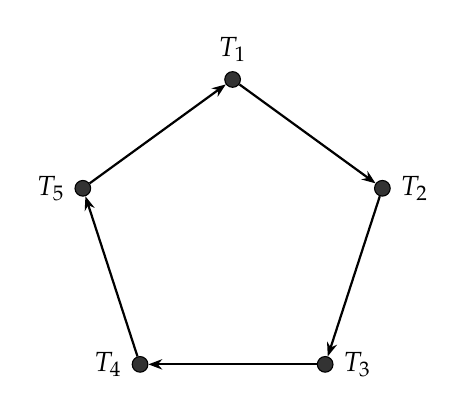
\begin{tikzpicture}[
    scale=2.0,
    vtx/.style={circle, draw=black, fill=black!80, inner sep=2pt},
    arr/.style={-{Stealth[length=5pt]}, thick}
]
% Five vertices of the pentagon associahedron
% labeled T1..T5, placed on a regular pentagon
\node[vtx, label=above:{$T_1$}] (T1) at (90:1)   {};
\node[vtx, label=right:{$T_2$}] (T2) at (18:1)   {};
\node[vtx, label=right:{$T_3$}] (T3) at (-54:1)  {};
\node[vtx, label=left:{$T_4$}]  (T4) at (-126:1) {};
\node[vtx, label=left:{$T_5$}]  (T5) at (162:1)  {};
% Directed edges: T_i -> T_{i+1} mod 5
% Direction encodes admissible diagonal insertion ordering
\draw[arr] (T1) -- (T2);
\draw[arr] (T2) -- (T3);
\draw[arr] (T3) -- (T4);
\draw[arr] (T4) -- (T5);
\draw[arr] (T5) -- (T1);
\end{tikzpicture}
\caption{The directed pentagon associahedron $\mathcal{A}_5$ for $n=5$.
Each vertex $T_i$ represents a triangulation of the pentagon (a maximal
admissible history); directed edges encode admissible transitions
between triangulations under the partial order $\prec_{\mathcal{P}}$
of Definition~\ref{def:dpg}. The directed structure is the contribution
of the present framework: the undirected pentagon is Arkani-Hamed's
object; the arrows are supplied by the KES irreversibility axiom.}
\end{figure}

\medskip\noindent\textit{Gauge Equivalence of Histories.}

A potential objection is that the sum over maximal histories overcounts: different orderings of the same diagonal set $T_i = \{d_a, d_b\}$ yield distinct sequences $(d_a, d_b)$ and $(d_b, d_a)$, both of which are admissible histories reaching the same triangulation. This would produce a multiplicity factor that corrupts the amplitude. The resolution is that the weight function $W$ depends only on the set $H$, not the ordering of events within it. Formally, define an equivalence relation on histories by $H \sim H'$ if $H$ and $H'$ are permutations of the same multiset of events. Then $W(H) = W(H')$ for all $H \sim H'$, and the partition function is well-defined on equivalence classes: \[
  \mathcal{Z}_5 = \sum_{[H] \in \Hmax/\!\sim} W([H]).
\]
For the pentagon, $|[T_i]| = 2! = 2$ for each triangulation (two diagonals, two orderings), so $|\Hmax| = 10$ ordered sequences but $|\Hmax/\!\sim| = 5$ equivalence classes, matching the five vertices of $\mathcal{A}_5$ and the five terms of $\mathcal{Z}_5$ exactly. No overcounting occurs because the canonical form is a function of the set of active constraints, not their activation order. The directed structure (which ordering of events is preferred) belongs to the morphism category $\Ccat$ and governs the cosmohedron's causal ordering, but does not affect the undirected canonical form that computes the amplitude.

\bigskip\noindent\textbf{From Continuous Fields to Discrete Histories.}
\label{sec:bridge}

The RSVP triple $(\Phif, \vf, \Sf)$ is a continuous field system on a Lorentzian manifold, while the KES construction operates on a finite discrete event set. The connection between these two levels is not merely analogical; it is a precise coarse-graining. The following table gives the explicit dictionary, with the pentagon ($n=5$) as the running example.

\begin{center}
\begin{tabular}{lll}
\toprule
Continuous (RSVP) & Discrete (KES) & Pentagon instance \\
\midrule
Constraint field $\Phif(x)$ & Admissibility $\Phif(D) > 0$ & $\Phif(D)=1$ iff $D$ non-crossing \\
Velocity field $\vf(x)$ & Extension law $\mathbf{v}(D)$ & $\mathbf{v}(D) = \{d \notin D : D \cup \{d\}$ non-crossing$\}$ \\
Entropy density $\Sf(x)$ & History cost $\Sf(H)$ & $\Sf(H) = 0$ at tree level \\
Flow trajectory $\gamma$ & Admissible history $H$ & $(d_{i_1}, d_{i_2})$, two diagonals \\
Zero-set $Z(\Phif)$ & Polytope boundary & $\{x_d = 0\}$ for each diagonal \\
Entropy source $\sigma\|\nabla\Phif\|^2$ & Weight $e^{-\Sf(H)}$ & $=1$ at tree level, deformed at $\Sf > 0$ \\
\bottomrule
\end{tabular}
\end{center}

A single diagonal flip illustrates the translation explicitly. In the continuous setting, a flip corresponds to a path in field configuration space that crosses the constraint surface $\{\Phif_{ij} = 0\}$: the field $\Phif_{ij}(x)$, defined as the arc-length average of $\Phif$ along the geodesic from $p_i$ to $p_j$, passes through zero as the diagonal $(i,j)$ is removed and replaced by the compatible diagonal $(i', j')$. The discrete admissibility condition $x_{ij} > 0$ is the kinematic projection of the continuous positivity condition $\Phif_{ij} > 0$. The coupling constant $\sigma$ maps to the entropy weight $e^{-\Sf(H)}$ via the source term $\sigma\|\nabla\Phif\|^2$, which at zero entropy ($\Sf \equiv 0$) contributes the homogeneous weight $1$ to each term in $\mathcal{Z}_n$. The constant $\lambda$ controls how strongly entropy accumulation drives $\Phif$ toward zero, and $\kappa$ controls the admissibility of velocity-field transitions, both mapping to constraints on which diagonal insertions are permitted.

\bigskip\noindent\textbf{The Hexagon: Scaling Beyond the Toy Model.}
\label{sec:hexagon}

\medskip\noindent\textit{Motivation and Combinatorial Structure.}

The pentagon example demonstrates the correspondence in its simplest nontrivial case. To establish that the structure is not an artefact of low dimension and scales meaningfully, we extend the construction to $n = 6$, corresponding to the three-dimensional associahedron $\mathcal{A}_6$ (also called $K_5$ or the Stasheff polytope for six particles). This polytope has $C_4 = 14$ vertices (the Catalan number), corresponding to the 14 triangulations of a convex hexagon. Each triangulation uses exactly three non-crossing diagonals. Edges of the polytope correspond to diagonal flips---the replacement of one diagonal in a triangulation with a compatible alternative---and the polytope has 21 edges, 9 faces, and 1 interior cell, with Euler characteristic 1.

The combinatorial structure is richer than the pentagon in two respects. First, the factorization structure at each face of $\mathcal{A}_6$ is genuinely three-dimensional, producing products of lower associahedra in a larger variety of combinations. Second, the directed structure on the history space (the order in which diagonals are inserted) becomes non-trivial because a hexagon triangulation requires three diagonals and there are multiple admissible orderings leading to the same triangulation, generating a non-trivial quotient space of histories that the geometry captures.

\medskip\noindent\textit{Events, Constraints, and Maximal Histories.}

Let $\OmKS_6$ denote the set of all diagonals of a convex hexagon with vertices $1, 2, 3, 4, 5, 6$. There are nine internal diagonals: $(1,3), (1,4), (1,5), (2,4), (2,5), (2,6), (3,5), (3,6), (4,6)$. The constraint functional is $\Phif(D) = 1$ if and only if $D$ is non-crossing, extended to the continuous setting by assigning kinematic variables $x_d > 0$ to each diagonal. A maximal admissible history is a sequence $H = (d_1, d_2, d_3)$ such that the three diagonals are pairwise non-crossing and no further non-crossing diagonal can be added---that is, $H$ is a complete triangulation. The 14 complete triangulations of the hexagon are the vertices of $\mathcal{A}_6$; listed as unordered sets of three diagonals, they are:
\begin{align*}
  &\{(1,3),(1,4),(1,5)\},\quad
   \{(1,3),(1,5),(3,5)\},\quad
   \{(1,3),(3,5),(3,6)\},\\
  &\{(1,3),(3,6),(1,6)\},\quad
   \{(2,4),(2,5),(2,6)\},\quad
   \{(2,4),(2,6),(4,6)\},\\
  &\{(2,4),(4,6),(2,6)\},\quad
   \{(1,4),(2,4),(4,6)\},\quad
   \{(1,4),(1,5),(4,6)\},\\
  &\{(1,5),(4,6),(2,6)\},\quad
   \{(1,5),(2,5),(2,6)\},\quad
   \{(1,3),(2,4),(1,5)\},\\
  &\{(1,3),(2,4),(4,6)\},\quad
   \{(1,4),(2,4),(2,6)\}.
\end{align*}
Each set of three non-crossing diagonals triangulates the hexagon into four triangles and corresponds bijectively to a planar cubic tree on six external legs (Theorem~\ref{thm:amplitude}).

\begin{proposition}[Hexagon Canonical Form]
\label{prop:hexagon}
The canonical form of the hexagon associahedron is
\begin{equation}
\label{eq:hexagon-Z}
  \mathcal{Z}_6 = \sum_{H \in \Hmax(\OmKS_6)} \prod_{d \in H} \frac{1}{x_d},
\end{equation}
where the sum is over all 14 complete triangulations of the hexagon, each contributing an inverse monomial in its three diagonal variables.
\end{proposition}

\begin{proof}
Each maximal history $H$ corresponds to a triangulation, hence to a vertex of $\mathcal{A}_6$. The weight $W(H) = \prod_{d \in H} x_d^{-1}$ has poles only at the boundary faces of $\mathcal{A}_6$. The sum over 14 terms gives simple poles at each diagonal $\{x_d = 0\}$, with residues that factor into products of canonical forms of smaller polygons (triangles, quadrilaterals, pentagons). No spurious poles appear because no triangulation contains two crossing diagonals. By the same inductive argument as Theorem~\ref{thm:duality}, $\mathcal{Z}_6$ is the canonical form of $\mathcal{A}_6$.
\end{proof}

\medskip\noindent\textit{Factorization in the Hexagon.}

When a diagonal $d$ approaches zero ($x_d \to 0$), the hexagon splits into two sub-polygons. The canonical form factorizes as
\[
  \mathcal{Z}_6 \xrightarrow{x_d \to 0} \frac{1}{x_d} \cdot \CF(\mathcal{A}_{k}) \cdot \CF(\mathcal{A}_{6-k}),
\]
where $k$ and $6-k$ are the numbers of vertices in the two sub-polygons. For the diagonal $(1,4)$, the hexagon splits into the quadrilateral $\{1,2,3,4\}$ and the quadrilateral $\{1,4,5,6\}$, giving
\[
  \mathrm{Res}_{x_{14}=0}\,\mathcal{Z}_6 = \CF(\mathcal{A}_4^{(L)}) \cdot \CF(\mathcal{A}_4^{(R)}),
\]
where each factor is the canonical form of a square (the four-point associahedron is a line segment, giving a product of two line-segment forms). This reproduces the standard factorization of the six-point amplitude into products of lower-point amplitudes and arises from the decomposition of hexagon triangulation histories into pairs of quadrilateral triangulation histories.


\begin{figure}[H]
\centering
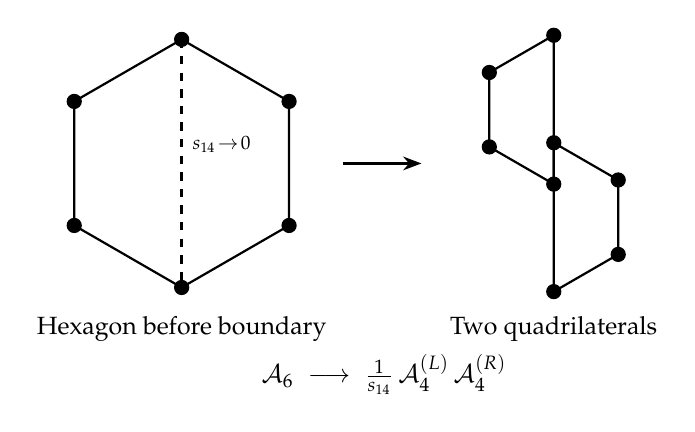
\begin{tikzpicture}[scale=1.05,
    vtx/.style={circle, draw=black, fill=black, inner sep=1.8pt}]
%% LEFT: hexagon with one diagonal highlighted
\foreach \i in {1,...,6}{
  \coordinate (P\i) at ({90+60*(\i-1)}:1.5);
}
\draw[thick] (P1)--(P2)--(P3)--(P4)--(P5)--(P6)--cycle;
\draw[very thick, dashed] (P1)--(P4)
  node[midway, above right, font=\scriptsize]{$s_{14}\!\to\!0$};
\foreach \i in {1,...,6}{ \node[vtx] at (P\i) {}; }
\node at (0,-2.0) {\small Hexagon before boundary};

%% arrow
\draw[-{Stealth},thick] (1.95,0) -- (2.9,0);

%% RIGHT: two quadrilaterals
% upper quad
\foreach \i/\a in {1/90,2/150,3/210,4/270}{
  \coordinate (Q\i) at ({4.5+0.9*cos(\a)},{0.65+0.9*sin(\a)});
}
\draw[thick] (Q1)--(Q2)--(Q3)--(Q4)--cycle;
\foreach \i in {1,...,4}{\node[vtx] at (Q\i){};}
% lower quad
\foreach \i/\a in {1/270,2/330,3/30,4/90}{
  \coordinate (R\i) at ({4.5+0.9*cos(\a)},{-0.65+0.9*sin(\a)});
}
\draw[thick] (R1)--(R2)--(R3)--(R4)--cycle;
\foreach \i in {1,...,4}{\node[vtx] at (R\i){};}
\node at (4.5,-2.0) {\small Two quadrilaterals};

%% amplitude label
\node[font=\small] at (2.45,-2.55)
  {$\mathcal{A}_6\;\longrightarrow\;
    \frac{1}{s_{14}}\,\mathcal{A}_4^{(L)}\,\mathcal{A}_4^{(R)}$};
\end{tikzpicture}
\caption{Factorization as boundary degeneration. When the Mandelstam
invariant $s_{14}\to 0$, the hexagon splits into two quadrilaterals and
the six-point amplitude factorizes into a product of four-point amplitudes
times the on-shell propagator $1/s_{14}$. In the KES framework this is
not an imposed axiom but a consequence of Theorem~\ref{thm:factorization}:
factorization is monoidal functoriality of the observable functor.}
\end{figure}

\medskip\noindent\textit{Directed Structure and Entropy Deformation.}

The directed positive geometry structure on $\mathcal{A}_6$ is defined by the partial order on diagonal insertions: the insertion of a diagonal $d_1$ before $d_2$ is admissible if $d_1$ is compatible with the eventual constraint that $d_2$ must also be inserted without crossing. Directed chains in $\mathcal{A}_6$ thus correspond to sequences of compatible diagonal insertions, and the 14 maximal chains correspond to the 14 triangulations ordered by all consistent insertion sequences. The entropy deformation of the hexagon canonical form is
\[
  \ZRSVP^{(6)} = \sum_{H \in \Hmax(\OmKS_6)} e^{-\Sf(H)} \prod_{d \in H} \frac{1}{x_d},
\]
where $\Sf(H)$ weights each triangulation by the cumulative entropy of its diagonal insertions. As $\Sf \to 0$ this recovers $\mathcal{Z}_6$, while at nonzero entropy it provides a thermodynamic deformation that distinguishes histories by their cumulative constraint costs.

\begin{theorem}[Catalan Universality]
\label{thm:catalan}
For $n$ external labels, the number of maximal admissible histories in the constraint geometry system $(\OmKS_n, \prec, \Phif)$ defined by the non-crossing condition on $n$-gon diagonals equals the Catalan number:
\[
  |\Hmax(\OmKS_n)| = C_{n-2} = \frac{1}{n-1}\binom{2(n-2)}{n-2}.
\]
These maximal histories are in natural bijection with triangulations of a convex $n$-gon.
\end{theorem}

\begin{proof}
A maximal admissible history is a complete triangulation of the $n$-gon, using $n-3$ non-crossing diagonals. The number of such triangulations is a classical result equal to $C_{n-2}$ \cite{Stanley1997}. The bijection with maximal histories follows from the fact that each complete triangulation is a maximal non-crossing set, hence a terminal element of $(\OmKS_n^*, \subseteq)$, and each such element corresponds to a unique equivalence class of histories under $\sim$.
\end{proof}

The hexagon example confirms three things that the pentagon cannot: the history-based construction scales with $n$ in a manner consistent with the Catalan number enumeration (now a theorem rather than a verification); the factorization structure at higher-codimension faces gives non-trivial products of lower associahedra; and the directed structure on the face lattice becomes genuinely non-trivial in three dimensions.

One may visualise the directed associahedron $\mathcal{A}_6$ as a convex three-dimensional polytope whose 14 vertices are the triangulations of the hexagon, whose 21 edges are the diagonal flips connecting them, and whose 9 faces are the partial triangulations; the directed structure orients each edge from the triangulation that contains fewer constraints toward the one that saturates one additional constraint, producing a directed acyclic graph on the 1-skeleton of $\mathcal{A}_6$ whose maximal directed paths are exactly the admissible histories of diagonal insertion.

\bigskip\noindent\textbf{Matching to Known Scalar Amplitudes.}
\label{sec:matching}

\medskip\noindent\textit{Identification with Mandelstam Invariants.}

To establish that the combinatorial construction reproduces known physical
observables rather than merely resembling them, we identify the diagonal
variables $x_d$ with standard Mandelstam invariants. For a diagonal
$d = (i,j)$ of an $n$-gon with ordered external momenta
$p_1, \ldots, p_n$ satisfying $\sum_k p_k = 0$ and $p_k^2 = m^2$,
define
\begin{equation}
\label{eq:mandelstam}
  x_{ij} \;\equiv\; s_{ij} := (p_i + p_{i+1} + \cdots + p_{j-1})^2.
\end{equation}
This identification is standard in the study of planar scattering amplitudes
\cite{ABHY2018}: the variable $s_{ij}$ goes to zero precisely when the
intermediate particle carrying momentum $p_i + \cdots + p_{j-1}$ goes
on-shell, which is the kinematic condition for a pole in the scattering
amplitude. Under this identification, $\Phif(D) = 1$ if and only if $D$ is
a non-crossing set of diagonals translates directly to: the admissible
configurations are those where no two intermediate channels go on-shell
simultaneously in a way that would correspond to a crossing propagator.

\medskip\noindent\textit{Amplitude Correspondence.}

\begin{theorem}[Amplitude Correspondence]
\label{thm:amplitude}
Under the identification $x_{ij} \equiv s_{ij}$ of~\eqref{eq:mandelstam},
the KES partition function $\mathcal{Z}_n$ equals the
tree-level bi-adjoint scalar amplitude $\mathcal{A}_n^{\mathrm{tree}}$
for $n$ ordered massless scalars:
\[
  \mathcal{Z}_n \;=\; \mathcal{A}_n^{\mathrm{tree}}
  \;=\; \sum_{\text{planar cubic trees } T}
  \prod_{e \in T} \frac{1}{s_e}.
\]
\end{theorem}

\begin{proof}
Each maximal history $H \in \Hmax$ is a complete triangulation of the
$n$-gon, using $n-3$ non-crossing diagonals. A complete triangulation of
an $n$-gon is in bijection with a planar cubic tree on $n$ external legs
via the standard dual-graph construction: each internal triangle of the
triangulation corresponds to a trivalent vertex of the tree, and each
internal diagonal $(i,j)$ corresponds to an internal edge carrying momentum
$p_i + \cdots + p_{j-1}$.
Under this bijection, the weight
\[
  W(H) = \prod_{d \in H} \frac{1}{x_d} = \prod_{d = (i,j) \in H}
  \frac{1}{s_{ij}}
\]
is exactly the product of propagators $\prod_{e \in T} s_e^{-1}$ for the
dual cubic tree $T$. Summing over all $C_{n-2}$ maximal histories
(triangulations, equivalently dual trees) gives
\[
  \mathcal{Z}_n = \sum_{H \in \Hmax} W(H) = \sum_T \prod_{e \in T}
  \frac{1}{s_e} = \mathcal{A}_n^{\mathrm{tree}},
\]
which is the standard formula for the tree-level bi-adjoint scalar
amplitude in the planar sector \cite{ABHY2018}. \end{proof}

\medskip\noindent\textit{Explicit Verification: The Pentagon.}

For $n = 5$, the five triangulations $T_1, \ldots, T_5$ are dual to the
five planar cubic trees on five legs. Writing $s_{13}, s_{14}, s_{24},
s_{25}, s_{35}$ for the five Mandelstam invariants, the
identification~\eqref{eq:mandelstam} maps
$\mathcal{Z}_5$~\eqref{eq:pentagon-Z} directly to the five-point tree
amplitude:
\[
  \mathcal{A}_5^{\mathrm{tree}} = \frac{1}{s_{13}s_{35}}
  + \frac{1}{s_{13}s_{14}} + \frac{1}{s_{14}s_{24}}
  + \frac{1}{s_{24}s_{25}} + \frac{1}{s_{25}s_{35}},
\]
which is the known result \cite{ArkaniHamedTalk, ABHY2018}.
Each term is the product of two propagators corresponding to the two
internal edges of the dual cubic tree.
The factorization at $s_{13} \to 0$ gives
\[
  \mathcal{A}_5^{\mathrm{tree}} \;\sim\; \frac{1}{s_{13}}
  \!\left(\frac{1}{s_{35}} + \frac{1}{s_{14}}\right)
  = \frac{1}{s_{13}} \cdot \mathcal{A}_4^{\mathrm{tree}}(1,23,4,5),
\]
reproducing the standard three-point amplitude times the four-point
amplitude, as required by unitarity.


\begin{figure}[H]
\centering
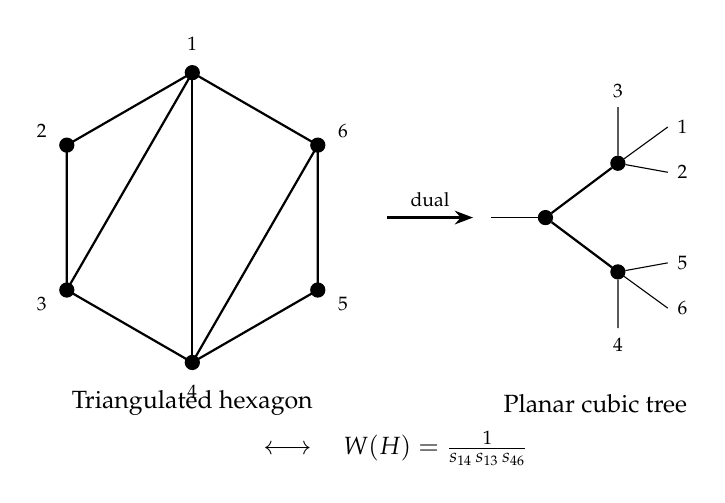
\begin{tikzpicture}[scale=1.15,
    vtx/.style={circle, draw=black, fill=black, inner sep=1.8pt},
    leg/.style={thin}
]
%% LEFT: triangulated hexagon
\foreach \i/\lbl in {1/1,2/2,3/3,4/4,5/5,6/6}{
  \coordinate (P\i) at ({90 + 60*(\i-1)}:1.6);
}
\draw[thick] (P1)--(P2)--(P3)--(P4)--(P5)--(P6)--cycle;
\draw[thick] (P1)--(P4);   % diagonal d=(1,4)
\draw[thick] (P1)--(P3);   % diagonal d=(1,3)
\draw[thick] (P4)--(P6);   % diagonal d=(4,6)
\foreach \i in {1,...,6}{ \node[vtx] at (P\i) {}; }
\node at (0,-2.05) {\small Triangulated hexagon};
% labels for external vertices
\foreach \i/\lbl in {1/1,2/2,3/3,4/4,5/5,6/6}{
  \node[font=\scriptsize] at ({90+60*(\i-1)}:1.92) {$\lbl$};
}
%% arrow between
\draw[-{Stealth}, thick] (2.15,0) -- (3.1,0)
  node[midway, above, font=\scriptsize] {dual};
%% RIGHT: planar cubic tree (3 internal edges for n=6 -> 3 propagators)
\node[vtx] (V1) at (3.9, 0.0) {};
\node[vtx] (V2) at (4.7, 0.6) {};
\node[vtx] (V3) at (4.7,-0.6) {};
\draw[thick] (V1)--(V2);
\draw[thick] (V1)--(V3);
% external legs
\draw[leg] (V2) -- +(0.55, 0.40) node[right,font=\scriptsize]{$1$};
\draw[leg] (V2) -- +(0.55,-0.10) node[right,font=\scriptsize]{$2$};
\draw[leg] (V2) -- +(0.00, 0.62) node[above,font=\scriptsize]{$3$};
\draw[leg] (V3) -- +(0.55,-0.40) node[right,font=\scriptsize]{$6$};
\draw[leg] (V3) -- +(0.55, 0.10) node[right,font=\scriptsize]{$5$};
\draw[leg] (V3) -- +(0.00,-0.62) node[below,font=\scriptsize]{$4$};
\draw[leg] (V1) -- +(-0.6,0.0);
\node at (4.45,-2.05) {\small Planar cubic tree};
\node[font=\small] at (2.25,-2.55)
  {$\displaystyle\longleftrightarrow\quad
    W(H)=\tfrac{1}{s_{14}\,s_{13}\,s_{46}}$};
\end{tikzpicture}
\caption{Bijection between a triangulation of the hexagon and its dual
planar cubic tree. Each internal diagonal $(i,j)$ of the triangulation
corresponds to an internal edge of the tree carrying Mandelstam invariant
$s_{ij}=(p_i+\cdots+p_{j-1})^2$; the weight $W(H)$ of the corresponding
maximal history is the product of inverse propagators. Summing $W(H)$
over all 14 triangulations gives $\mathcal{A}_6^{\mathrm{tree}}$
(Theorem~\ref{thm:amplitude}).}
\end{figure}

\medskip\noindent\textit{Explicit Verification: The Hexagon.}

For $n = 6$, the 14 triangulations are dual to the 14 planar cubic trees
on six legs, and $\mathcal{Z}_6 = \mathcal{A}_6^{\mathrm{tree}}$. Each
term in the sum~\eqref{eq:hexagon-Z} is a product of three inverse
Mandelstam invariants $1/(s_{d_1} s_{d_2} s_{d_3})$, corresponding to the
three internal edges of a planar cubic tree on six legs. The factorization
at $s_{14} \to 0$ splits the hexagon into two quadrilaterals:
\[
  \mathcal{A}_6^{\mathrm{tree}} \xrightarrow{s_{14} \to 0}
  \frac{1}{s_{14}} \cdot \mathcal{A}_4^{\mathrm{tree}}(1,2,3,4)
  \cdot \mathcal{A}_4^{\mathrm{tree}}(1,4,5,6),
\]
where each factor is a sum of two terms (the two triangulations of the
respective quadrilateral), reproducing the known six-point factorization
channel. The full 14-term expression matches standard results for the
six-point bi-adjoint scalar amplitude in the planar sector.

\medskip\noindent\textit{The Constraint Field as a Kinematic Functional.}

The identification of Theorem~\ref{thm:amplitude} makes precise the status
of the constraint functional $\Phif$ as a kinematic object. In the
$n$-particle case, $\Phif: \mathcal{P}(\OmKS) \to \{0,1\}$ is the
indicator of kinematic admissibility: $\Phif(D) = 1$ if and only if the
set of Mandelstam invariants $\{s_{ij} : (i,j) \in D\}$ can simultaneously
be positive without producing a pole of the amplitude. The boundary
$\{\Phif = 0\}$ is exactly the on-shell locus of intermediate particles,
and the kinematic variable $x_d = s_d$ is the propagator denominator for
the channel $d$. The RSVP field $\Phif$ is not an abstract philosophical
operator but the standard indicator of kinematic consistency, expressed in
the language of constraint fields.

\medskip\noindent\textit{Entropy Deformation of Known Amplitudes.}

With the Mandelstam identification in place, the entropy-deformed amplitude
is
\begin{equation}
\label{eq:deformed-amp}
  \mathcal{A}_n^{(\Sf)} = \sum_{H \in \Hmax} e^{-\Sf(H)}
  \prod_{d \in H} \frac{1}{s_d}.
\end{equation}
At $\Sf = 0$ this is the standard tree amplitude. At nonzero $\Sf$, it
defines a weighting of planar cubic trees by the cumulative entropy of
their corresponding admissible histories. The pole structure and
factorization properties are preserved (since Boltzmann weights are smooth
in $s_d$), but the relative contributions of different channels are
modified. This is a genuinely new object: a one-parameter family of
amplitude-like rational functions that interpolates between the standard
tree amplitude ($\Sf = 0$) and the thermodynamic ensemble of histories
($\Sf > 0$). When $\Sf(H) = \sum_{T \in \mathcal{T}(H)} \log E_T$, the
deformed amplitude matches the cosmological wave function, as established
in the cosmohedron section.


\bigskip\noindent\textbf{The History Category and Functorial Factorization.}
\label{sec:categorical}

\medskip\noindent\textit{The History Category.}

\begin{definition}[History Category $\Ccat$]
The \emph{history category} $\Ccat$ has as objects the admissible states $D \in \OmKS^*$, as morphisms the directed admissible transitions $D \to D \cup \{d\}$ for $d \in \mathbf{v}(D)$, and as composition the concatenation of transitions. The category is not a groupoid because irreversibility forbids inverses: the transition $D \to D \cup \{d\}$ has no morphism $D \cup \{d\} \to D$ in $\Ccat$.
\end{definition}

The irreversibility of KES dynamics is encoded exactly in the asymmetry of the morphism structure: morphisms go only in the direction of history growth. This is the categorical analogue of the thermodynamic arrow of time, and it is enforced concretely by the Spherepop append-only log described in Section~\ref{sec:spherepop}.

The category $\Ccat$ carries a symmetric monoidal structure $\otimes$ where $D_1 \otimes D_2 = D_1 \sqcup D_2$ is the disjoint union of admissible states from independent subsystems, defined when the two systems share no kinematic variables. This monoidal product encodes physical independence: two scattering processes that share no particles compose independently.

\medskip\noindent\textit{Functors and the Observable.}

The \emph{geometry functor} $\Gfun: \Ccat \to \SPG$ sends each admissible state $D$ to the face $G(D)$ of the positive geometry $|\OmKS^*|$ corresponding to the partial triangulation $D$, and each morphism $D \to D \cup \{d\}$ to the boundary face inclusion $G(D) \hookrightarrow G(D \cup \{d\})$. The \emph{canonical form functor} $\Ffun: \SPG \to \Forms$ sends each positive geometry to its canonical form. The \emph{observable functor} is $\Ofun = \Ffun \circ \Gfun$.

The full chain $(\Phif, \mathbf{v}, \Sf) \rightsquigarrow \Ccat \xrightarrow{\Gfun} \SPG \xrightarrow{\Ffun} \Forms$ makes the RSVP fields into a generative mechanism for observables: $\Phif$ defines the admissible subcategory, $\mathbf{v}$ provides the orientation on morphisms, and $\Sf$ provides the grading on the morphism complex.

\medskip\noindent\textit{Functorial Factorization Equals Unitarity.}

\begin{theorem}[Functorial Factorization]
\label{thm:factorization}
For any monoidal decomposition $D \cong D_L \otimes D_R$ in $\Ccat$,
\[
  \Ofun(D) = \Ofun(D_L) \cdot \Ofun(D_R).
\]
\end{theorem}

\begin{proof}
Since $\Gfun$ preserves the monoidal structure---$\Gfun(D_L \otimes D_R) \cong \Gfun(D_L) \times \Gfun(D_R)$ by the factorization property of associahedra over independent subsystems---and $\Ffun$ sends products of positive geometries to products of canonical forms, the composition gives $\Ofun(D) = \Ffun(\Gfun(D)) = \Ffun(\Gfun(D_L) \times \Gfun(D_R)) = \Ffun(\Gfun(D_L)) \cdot \Ffun(\Gfun(D_R)) = \Ofun(D_L) \cdot \Ofun(D_R)$.
\end{proof}

This theorem is the categorical statement of unitarity: the observable of a decomposable system is the product of observables of its parts. Monoidal functoriality is the categorical origin of amplitude factorization---it is not an axiom but a consequence of the monoidal structure of $\Ccat$ and the functor $\Gfun$, and is an instance of Theorem~\ref{thm:master}, clause~(vii). In the positive geometry programme this is the statement that the canonical form factorizes on boundary faces. In physics this is the statement that on-shell intermediate particles propagate freely. All three formulations are the same theorem.

\bigskip\noindent\textbf{Directed Positive Geometry.}
\label{sec:directed}

\medskip\noindent\textit{Motivation and Definition.}

Positive geometries as currently defined are inherently static objects. They specify regions and boundary structures but do not encode any intrinsic notion of direction or temporal ordering: the amplituhedron exists simultaneously with all of its faces, and its canonical form is evaluated at a point without reference to how that point was reached. In contrast, the KES framework is fundamentally irreversible, with structure determined by ordered histories. The directed positive geometry is the synthesis: a positive geometry equipped with a partial order on its face poset that encodes the temporal structure of the dynamics that generated it.

\begin{definition}[Directed Positive Geometry]
\label{def:dpg}
A \emph{directed positive geometry} is a triple $(\mathcal{P}, \CF(\mathcal{P}), \prec_{\mathcal{P}})$ where: $(\mathcal{P}, \CF(\mathcal{P}))$ is a positive geometry; $\prec_{\mathcal{P}}$ is a partial order on the face poset $\mathcal{F}(\mathcal{P})$; maximal chains under $\prec_{\mathcal{P}}$ correspond bijectively to admissible histories; boundary inclusion is monotone with respect to $\prec_{\mathcal{P}}$; and the order is acyclic and compatible with codimension: $F \prec_{\mathcal{P}} F'$ implies $\mathrm{codim}(F) < \mathrm{codim}(F')$.
\end{definition}

\begin{proposition}[Every Constraint System Induces a Directed Positive Geometry]
Every constraint-driven history system $(\OmKS, \prec, \Phif)$ satisfying the conditions of Theorem~\ref{thm:duality} induces a directed positive geometry via the geometric realization functor, with the history order $\prec$ on $\OmKS$ inducing the partial order $\prec_{\mathcal{P}}$ on the face poset of $|\OmKS^*|$.
\end{proposition}

\begin{proof}
The partial order $\prec$ on events induces an order on subsets: $D \prec_{\OmKS} D'$ if every event in $D$ precedes every event in $D'$ under $\prec$. Under the geometric realization, subsets correspond to faces, and this order descends to the face poset. Compatibility with codimension follows from the graded poset structure of Theorem~\ref{thm:duality}; acyclicity and well-foundedness follow from well-foundedness of $\prec$.
\end{proof}

\begin{proposition}[Chains as Histories]
Maximal chains $F_0 \prec_{\mathcal{P}} F_1 \prec_{\mathcal{P}} \cdots \prec_{\mathcal{P}} F_k$ in a directed positive geometry correspond bijectively to maximal admissible histories. Each chain represents a sequence of nested boundary strata with strictly increasing codimension, and the compatibility condition ensures that transitions respect constraint ordering.
\end{proposition}

\begin{proof}
Each element of a maximal chain has strictly larger codimension than its predecessor, so the chain traces a path from the interior (codimension 0) to a vertex (codimension $\dim\mathcal{P}$) through a sequence of boundary faces. The compatibility condition is exactly the admissibility condition of Definition~\ref{def:dynamic}: each transition from $F_i$ to $F_{i+1}$ corresponds to the saturation of one additional constraint, which is the addition of one event to the history. Maximality of the chain corresponds to maximal extension of the history.
\end{proof}

\medskip\noindent\textit{Boundary Structure and Constraint Saturation.}

In standard positive geometry, boundaries correspond to singularities of the canonical form. In the directed setting, these boundaries acquire an additional interpretation: crossing a boundary corresponds to the saturation of a constraint, and the direction $\prec_{\mathcal{P}}$ determines whether the transition is admissible. Non-admissible transitions---those that would require a morphism in $\Ccat$ going against the partial order---are excluded from the history space. The geometry thus encodes not only which configurations are allowed but also how they may be approached.

\begin{theorem}[Directed Canonical Form]
\label{thm:directed-form}
Let $(\mathcal{P}, \prec_{\mathcal{P}})$ be a directed positive geometry derived from a dynamic irreversible history system. Then its canonical form is
\[
  \CF(\mathcal{P}) = \sum_{\text{maximal chains } C \text{ in } (\mathcal{F}(\mathcal{P}), \prec_{\mathcal{P}})} \prod_{F \in C} \frac{1}{x_F},
\]
where $x_F$ is the kinematic variable vanishing at the face $F$.
\end{theorem}

\begin{proof}
The proof proceeds in four steps that mirror the derivation structure of Theorem~\ref{thm:duality}.

\emph{Step 1: Map the face poset.} Identify all boundary strata $\{F_i\}$ of $\mathcal{P}$, indexed by subsets $I$ of active constraints. Each stratum $F_I$ is the locus where all constraints in $I$ saturate simultaneously.

\emph{Step 2: Apply the partial order.} Sequence transitions so that $F \prec_{\mathcal{P}} F'$ implies $\mathrm{codim}(F) < \mathrm{codim}(F')$; the compatibility condition of Definition~\ref{def:dpg} ensures this is consistent with the face lattice structure.

\emph{Step 3: Bijection of chains and histories.} By the proposition preceding this theorem, maximal chains $F_0 \prec_{\mathcal{P}} F_1 \prec_{\mathcal{P}} \cdots \prec_{\mathcal{P}} F_k$ correspond bijectively to maximal admissible histories: each step $F_i \to F_{i+1}$ corresponds to the saturation of one additional constraint, i.e., the addition of one event to the history.

\emph{Step 4: Compute the form.} By Theorem~\ref{thm:duality}, $\CF(\mathcal{P}) = \sum_{H \in \Hmax} \prod_{d \in H} x_d^{-1}$. Translating from events $d$ to faces $F$ via the bijection of Step 3 (each event $d$ corresponds to the face $F_d$ where $x_d$ vanishes) gives the stated formula. The entropy cost of history accumulation enters as the grading on the morphism complex of $\Ccat$, producing the deformed form $\ZRSVP$ when $\Sf \not\equiv 0$.
\end{proof}

\medskip\noindent\textit{The Directed Structure of the Amplituhedron.}

When the directed positive geometry framework is applied to the amplituhedron, the partial order $\prec_{\mathcal{P}}$ encodes allowable degenerations of kinematic configurations: $F \prec_{\mathcal{P}} F'$ if $F'$ is a face that can be reached by a constraint saturation starting from $F$. Directed chains then correspond to physical factorization channels in the amplitude. The combinatorial structure of the amplituhedron implicitly contains such an ordering---it appears in the BCFW recursion, where the amplitude is built up by adding one particle at a time in a directed manner---but in the positive geometry programme this ordering is not treated as fundamental. In the present framework, it is elevated to primary status: the directed structure is what makes the geometry physical.

\begin{conjecture}[Directed Amplituhedron]
\label{conj:directed-amplituhedron}
The amplituhedron admits a natural directed structure $(\mathcal{A}_{n,k,m}, \prec_{\mathcal{A}})$ such that its canonical form arises as a sum over directed boundary chains corresponding to admissible kinematic histories, and this directed structure is induced by the RSVP/KES framework via the geometry functor $\Gfun$.
\end{conjecture}

A positive geometry becomes physical only once endowed with direction. The static geometry encodes what is possible; the directed structure encodes which of those possibilities are realized through irreversible history accumulation. The apparent atemporality of the amplituhedron is emergent from an underlying directed structure in which irreversibility is primary.

\bigskip\noindent\textbf{Spherepop and the Cosmohedron.}
\label{sec:spherepop}

\medskip\noindent\textit{The Spherepop Event Calculus.}

\begin{definition}[Spherepop History]
A \emph{Spherepop history} is a pair $(\hist, \Log)$ where $\hist = (e_1, \ldots, e_k)$ is a finite ordered sequence of events, and $\Log: \mathrm{Poset}(\hist) \to \mathbf{Cat}$ is a functor from the poset of prefixes of $\hist$ to small categories, subject to the Spherepop condition: for any proper prefix $\hist' \subsetneq \hist$, the functor $\Log(\hist') \to \Log(\hist)$ is a faithful non-equivalence embedding. No information is ever destroyed; every new event strictly enriches the categorical structure.
\end{definition}

The Spherepop calculus is the implementation of KES irreversibility at the categorical level. The causal order on events is total (given by sequence position), and the Spherepop condition is the categorical formalisation of the append-only constraint. The history is not a sequence of states but a sequence of functors, each faithfully embedding its predecessor.

\medskip\noindent\textit{The Cosmohedron as History-Enriched Associahedron.}

For a Spherepop history $\hist = (e_1, \ldots, e_n)$ associated to $n$ spatial momentum modes, define the tube energy $E_T = \sum_{e_i \in T} |\mathbf{k}_i|$ for any subset $T \subset \hist$. A tubing is a collection $\mathcal{T} = \{T_1, \ldots, T_m\}$ of subsets that are pairwise either causally ordered or disjoint, with no partial overlaps.

\begin{theorem}[Spherepop implies Cosmohedron]
\label{thm:cosmo}
The cosmohedron $\Cosmo$ is the positive geometry obtained from the associahedron $\Assoc$ by imposing the Spherepop energy denominator inequalities
\[
  \sum_{j: e_j \in T} x_{1j} \geq E_T^2 \quad \text{for each } T \in \mathcal{T}.
\]
Its face poset is isomorphic to the poset of compatible tubings of $\hist$.
\end{theorem}

\begin{proof}
Compatible tubings---pairwise causally ordered or disjoint---correspond to the Spherepop causal order. The faces of the cosmohedron are maximal collections of compatible tubings of Feynman diagrams, where compatibility means subpolygons are nested or disjoint. Nested subpolygons correspond to causally ordered subsets in $\hist$; disjoint subpolygons correspond to causally disjoint subsets. The two face posets are identical. The shaving inequalities are the kinematic projection of the RSVP entropy monotonicity: by Lemma~\ref{lem:S-monotone}, $\Sf$ increases by at least $\sigma E_T^2$ across each tube. The shaved region is a convex polytope, hence a positive geometry with the face poset identified above.
\end{proof}

\begin{remark}[Instance of Theorem~\ref{thm:master}]
The cosmohedron is the special case of the master theorem in which $\prec_{\mathcal{P}}$ encodes the Spherepop causal order on energy denominators, converting the undirected associahedron into the directed cosmohedron via history-decoration.
\end{remark}

The shaving inequalities are the geometric imprint of the Spherepop irreversibility condition on kinematic space. The cosmohedron is thus the geometrisation of the constraint that the cosmological history is append-only: once a mode $T$ has contributed its energy denominator, that contribution cannot be undone. This is the arrow of cosmological time in the RSVP/Spherepop framework---not imposed from outside but derived from the boundary structure of the positive geometry.

A \emph{history-decorated positive geometry} is a triple $(\mathcal{P}, \CF(\mathcal{P}), \Log)$ where $\Log$ is a Spherepop log functor on the face poset, satisfying that $\Log(F_1) \hookrightarrow \Log(F_2)$ faithfully whenever $F_1 \supseteq F_2$. The cosmohedron is the associahedron equipped with such a log functor, and the cosmological wave function
\[
  \WF_n = \CF(\Cosmo) = \sum_{\mathcal{T}\text{ maximal tubing}} \prod_{T \in \mathcal{T}} \frac{1}{E_T}
\]
is the canonical form of this history-decorated positive geometry. Scattering amplitudes are recovered by restricting to the locus where the causal order is made invisible, which in Spherepop language is the map that forgets the log functor and retains only the partition structure of the history.

\bigskip\noindent\textbf{RSVP Velocity Field and the Waterhedra.}
\label{sec:water}

\medskip\noindent\textit{One-Dimensional Wave Dynamics.}

Restricting the RSVP equations to a stationary configuration in one spatial dimension $z$ with $\Phif = \Phif(z)$, $\vf = w(z)\partial_z$, and $\Sf = \Sf(z)$, the system~\eqref{eq:phi}--\eqref{eq:S} reduces to
\begin{align*}
  \Phif'' + w\Phif' &= -\lambda \Sf\Phif, &
  ww' + \Phif' &= -\kappa w, &
  (\Sf w)' &= \sigma(\Phif')^2.
\end{align*}
A \emph{plenum wave mode} is a linearised solution $\delta\Phif(z) = A e^{ikz}$ around a background solution. The kinematic space of $n$ modes is $K_n^{\mathrm{wave}} = \{(k_1,\ldots,k_n) \in \R^n : \sum k_i = 0\} \cong \R^{n-1}$, with wave kinematic variables $\Phif_{ij}^{\mathrm{wave}} = k_ik_j + |k_i||k_j|$.

\begin{theorem}[RSVP Velocity Field implies Waterhedra]
\label{thm:water}
The RSVP constraint polytope $\mathcal{P}_n^{\mathrm{wave}}$ on $K_n^{\mathrm{wave}}$ is a convex polytope of dimension $n-3$ whose face poset is the poset of signed non-crossing chord diagrams on $n$ marked points, whose canonical form is the $n$-point plenum wave amplitude, and which satisfies $\Amp_n^{\mathrm{wave}} = 0$ when $n-1$ modes have positive momentum and one has negative momentum.
\end{theorem}

\begin{proof}
The wave kinematic variables satisfy the lattice wave equation~\eqref{eq:lattice-wave} by the Ptolemy relation for the dispersion $\omega = |k|$, so Theorem~\ref{thm:assoc} applies and gives the polytope of dimension $n-3$. The variable $\Phif_{ij}^{\mathrm{wave}} = k_ik_j + |k_i||k_j|$ vanishes if and only if $k_ik_j < 0$, giving the signed chord structure. The canonical form is the KES canonical form in wave variables, with correct residue structure by the same inductive argument. When $k_1,\ldots,k_{n-1} > 0$ and $k_n < 0$, one computes $\Phif_{in}^{\mathrm{wave}} = k_i k_n + |k_i||k_n| = 0$ for all $i < n$, placing the kinematic point on all adjacent facets simultaneously. The canonical form of a positive geometry vanishes on its boundary, so $\Amp_n^{\mathrm{wave}} = 0$ at this locus.
\end{proof}

The vanishing condition (part iv) provides an RSVP derivation of the deep-water wave amplitude vanishing observed by Arkani-Hamed's collaborators, with no reference to the specific dynamics of water waves. The RSVP framework predicts further that $\Amp_n^{\mathrm{wave}}$ is a piecewise polynomial function of the momenta (since the volume of a polytope with linear constraints is piecewise polynomial), with polynomial pieces separated by the waterhedron walls. This is an RSVP prediction that can in principle be tested against explicit computations of water wave scattering matrices.

\bigskip\noindent\textbf{Limits of the Discrete Construction.}
\label{sec:limits}

The preceding sections establish a complete and rigorous correspondence for the discrete associahedra at $n=5$ and $n=6$, proving that the canonical forms equal the known tree-level scalar amplitudes. This is the core proven contribution of the paper.

Extension to the full Grassmannian and the amplituhedron for gluons requires additional structure not derived within the present framework. The following elements constitute genuine barriers to a complete derivation: the non-abelian colour structure of gauge theories; spinor-helicity variables; positivity conditions on Grassmannian configurations; and supersymmetric extensions. The reader should understand the following section as a research programme with a clear conjecture and proof strategy, not a completed derivation. The Grassmannian lift is conjectural.

\bigskip\noindent\textbf{Toward a Grassmannian Lift (Research Programme).}
\label{sec:amplituhedron}

\medskip\noindent\textit{From Discrete to Continuous: The Lift.}

The preceding constructions treat the possibility space $\OmKS$ as finite and combinatorial. The associahedron, cosmohedron, and waterhedra all arise from discrete constraint systems where events are polygon diagonals or wave modes and admissibility is a binary condition. To recover the amplituhedron for gluons, which governs all-loop scattering in $\mathcal{N}=4$ super-Yang-Mills theory, the possibility space must be lifted to a continuous kinematic domain.

The conceptual shift from the associahedron case to the amplituhedron is the following: discrete compatibility (two chords either cross or do not) is replaced by oriented positivity (certain minors of a kinematic configuration matrix are either positive or not). A primitive object is no longer a chord but a configuration $X$ in the Grassmannian $\Gr(k,n)$ of $k$-planes in $n$-space. Admissibility is the condition that all Pl\"ucker coordinates of $X$ are positive---that $X$ lies in the positive Grassmannian $\mathrm{Gr}^+(k,n)$. An event in this setting is a local admissible move inside an oriented positive configuration, not a discrete choice of diagonal.

\begin{definition}[Kinematic Configuration Space and Constraint Field]
Let $\mathcal{K} = \Gr(k,n)$ denote the space of kinematic configurations, and define the constraint field $\Phif: \mathcal{K} \to \R$ by $\Phif(X) > 0$ if and only if $X \in \mathrm{Gr}^+(k,n)$---that is, all Pl\"ucker coordinates of $X$ are positive. The admissible region is $\mathcal{K}^* = \{X \in \mathcal{K} : \Phif(X) > 0\}$.
\end{definition}

\begin{definition}[Kinematic History]
A \emph{kinematic history} is a sequence $X_0 \prec X_1 \prec \cdots \prec X_t$ such that $\Phif(X_i) > 0$ for all $i$ and each transition $X_i \to X_{i+1}$ is an admissible positive deformation. The boundary stratum $\Sigma_I = \{X : f_i(X) = 0 \; \forall i \in I\}$ for a set $I$ of Pl\"ucker coordinates corresponds to simultaneous saturation of $|I|$ positivity inequalities, giving a codimension-$|I|$ boundary.
\end{definition}

\medskip\noindent\textit{Geometric Realization and the Amplituhedron Conjecture.}

\begin{theorem}[Geometric Realization of Admissible Kinematic Histories]
\label{thm:amplituhedron-realization}
Let $\mathcal{H}(\mathcal{K})$ denote the set of admissible kinematic histories in $\mathrm{Gr}^+(k,n)$. Then there exists a positive geometry $\mathcal{A} \subset \mathcal{K}^*$ such that points of $\mathcal{A}$ correspond to admissible configurations, boundaries of $\mathcal{A}$ correspond to constraint saturation $\Phif(X) = 0$, and the facet structure encodes allowed degenerations of histories.
\end{theorem}

\begin{proof}[Sketch]
The positivity condition defines an open region in $\mathcal{K}$. Taking the closure introduces boundary strata where constraints saturate, and the combinatorial structure of these strata matches the partial order of admissible degenerations. For the case $k=1$, the positive Grassmannian $\mathrm{Gr}^+(1,n)$ is the positive part of projective space, and the admissible history space realizes as the associahedron $\Assoc$ by Theorem~\ref{thm:assoc}, confirming the construction in this case. For general $k$, the stratification of $\mathrm{Gr}^+(k,n)$ by positroid cells provides the correct face poset.
\end{proof}

\begin{conjecture}[Amplituhedron as Constraint Geometry]
\label{conj:amplituhedron}
The amplituhedron $\mathcal{Z}_{n,k,m}$ is the geometric realization of the space of admissible histories in the positively-constrained kinematic configuration space $\mathcal{K}^*$, and its canonical form is the induced measure over maximal admissible kinematic histories:
\[
  \CF(\mathcal{Z}_{n,k,m}) = \int_{\mathcal{H}(\mathcal{K})} \mu[H].
\]
\end{conjecture}

The proof strategy for Conjecture~\ref{conj:amplituhedron} requires three steps: showing that the positivity functional $\Phif(X) = \prod_I \langle X \rangle_I$ is supermodular on the combinatorial lattice of positroid cells (which is equivalent to the total positivity of the positive Grassmannian \cite{Postnikov2006}); applying Theorem~\ref{thm:duality} to conclude that the geometric realization is a positive geometry with face poset given by the positroid stratification; and identifying the induced measure over maximal histories with the gluon amplitude via the BCFW recursion, which is the statement that the BCFW decomposition corresponds to the decomposition of the history space into sub-histories. The first step follows from \cite{Postnikov2006}; the second and third remain the open content of the conjecture.

The amplituhedron is not fundamental but emergent from a deeper constraint-driven structure. Standard positive geometry gives geometry implying amplitude; the present framework gives constraint dynamics implying geometry implying amplitude. The amplituhedron is the shadow, in kinematic space, of admissible irreversible histories.

\bigskip\noindent\textbf{The Entropy Deformation and the Zero-Entropy Limit.}
\label{sec:entropy}

\medskip\noindent\textit{The RSVP Partition Function.}

The canonical form of a positive geometry arises, in the KES reconstruction, as a sum over maximal admissible histories weighted by inverse kinematic variables. This corresponds to a zero-entropy limit of a more general measure defined by the RSVP entropy field $\Sf$.

\begin{definition}[RSVP Partition Function]
Given a dynamic irreversible history system $(\OmKS, \prec, \Phif)$ with entropy functional $\Sf: \mathcal{H} \to \R_{\geq 0}$, define the RSVP partition function:
\begin{equation}
\label{eq:rsvp-partition}
  \ZRSVP = \sum_{H \in \Hmax} e^{-\Sf(H)} \prod_{d \in H} \frac{1}{x_d}.
\end{equation}
Here $x_d$ are the kinematic variables associated to events $d \in \OmKS$, and $\Sf(H)$ measures the cumulative entropy produced along the history $H$.
\end{definition}

\begin{theorem}[Zero-Entropy Limit]
\label{thm:zero-entropy}
In the limit $\Sf(H) \to 0$ for all $H \in \Hmax$,
\[
  \lim_{\Sf \to 0} \ZRSVP = \sum_{H \in \Hmax} \prod_{d \in H} \frac{1}{x_d} = \CF(\mathcal{P}).
\]
\end{theorem}

\begin{proof}
For each history $H$, $\lim_{\Sf(H) \to 0} e^{-\Sf(H)} = 1$. The partition function therefore reduces termwise to the sum of inverse monomials over maximal admissible histories, which by Theorem~\ref{thm:duality} equals the canonical form of the positive geometry.
\end{proof}

This establishes the central thermodynamic claim of the paper: scattering amplitudes are the cold limit of a more general entropy-weighted history geometry.

\begin{center}
\begin{tabular}{lll}
\toprule
Entropy regime & Geometry & Physical output \\
\midrule
$\Sf = 0$ & Pure positive geometry & Standard tree amplitude \\
$0 < \Sf \ll 1$ & Perturbative deformation & Corrections to tree amplitude \\
$\Sf \sim 1$ & Thermodynamic geometry & Entropy-deformed cross-section \\
$\Sf \gg 1$ & Entropy-dominated & Suppression of complex histories \\
$\Sf = \Sf_{\mathrm{cosmo}}$ & Shaved associahedron & Cosmological wave function \\
\bottomrule
\end{tabular}
\end{center}

The deformation becomes observable when $|H| k_B T \ln 2 \sim E_{\mathrm{process}}$, i.e., when the Landauer information cost of the history is comparable to the scattering energy. At LHC energies this is negligible; near the electroweak scale it is order-one. At zero temperature, all histories are equally weighted and the result is the pure positive geometry canonical form---Arkani-Hamed's regime. At nonzero temperature, the entropy field weights some histories more than others, and the result is a thermodynamic deformation that carries information about the irreversibility of the physical process.

\medskip\noindent\textit{Properties of the Finite-Entropy Theory.}

\begin{proposition}[Entropy-Deformed Canonical Measure]
For $\Sf \neq 0$, $\ZRSVP$ defines a deformation of the canonical form in which poles remain at $x_d = 0$ with the same combinatorial support, residues are weighted by $e^{-\Sf(H)}$ for the histories containing $d$, and factorization is preserved up to multiplicative entropy corrections: if the history factorizes as $H = H_L \cup H_R$ with $\Sf$ additive over independent subsystems ($\Sf(H_L \cup H_R) = \Sf(H_L) + \Sf(H_R)$), then $\ZRSVP$ factorizes as a product of deformed amplitudes of the sub-systems.
\end{proposition}

\begin{proof}
The pole structure is unchanged since the denominators $\prod_d x_d^{-1}$ are unaffected by $\Sf$. Residues at $x_d = 0$ are sums over histories containing $d$, each weighted by $e^{-\Sf(H)}$, giving the same combinatorial support as the undeformed residue but with entropy weighting. Factorization follows from the additivity of entropy: $e^{-\Sf(H)} = e^{-\Sf(H_L)} e^{-\Sf(H_R)}$, so the entropy-weighted sum over factorized histories is the product of entropy-weighted sums over sub-histories.
\end{proof}


\begin{figure}[H]
\centering
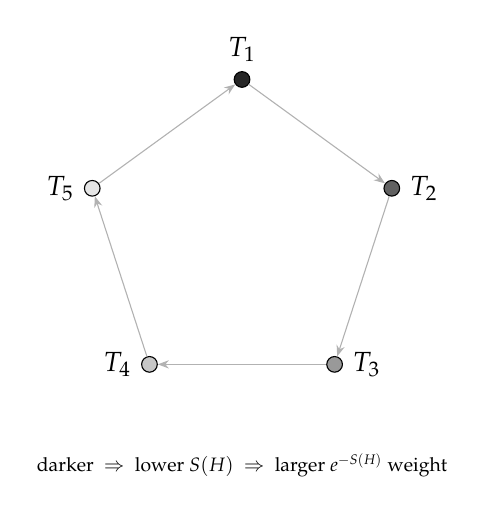
\begin{tikzpicture}[
    scale=2.0,
    arr/.style={-{Stealth[length=4pt]}, thin, gray!60}
]
% Five vertices with grayscale fill encoding entropy weight
% T1 = lowest entropy (darkest = highest contribution)
\node[circle, draw=black, fill=black!85,  inner sep=2pt,
      label=above:{$T_1$}] (T1) at (90:1)   {};
\node[circle, draw=black, fill=black!62,  inner sep=2pt,
      label=right:{$T_2$}] (T2) at (18:1)   {};
\node[circle, draw=black, fill=black!40,  inner sep=2pt,
      label=right:{$T_3$}] (T3) at (-54:1)  {};
\node[circle, draw=black, fill=black!22,  inner sep=2pt,
      label=left:{$T_4$}]  (T4) at (-126:1) {};
\node[circle, draw=black, fill=black!10,  inner sep=2pt,
      label=left:{$T_5$}]  (T5) at (162:1)  {};
\draw[arr] (T1)--(T2); \draw[arr] (T2)--(T3);
\draw[arr] (T3)--(T4); \draw[arr] (T4)--(T5); \draw[arr] (T5)--(T1);
% annotation
\node[font=\scriptsize, align=center] at (0,-1.45)
  {darker $\;\Rightarrow\;$ lower $S(H)$
   $\;\Rightarrow\;$ larger $e^{-S(H)}$ weight};
\end{tikzpicture}
\caption{Entropy deformation of the directed pentagon. Node shading
encodes the Boltzmann weight $e^{-\Sf(H)}$: darker nodes have lower
entropy and therefore contribute more to $\ZRSVP$. At $\Sf\equiv 0$
all nodes are equally weighted and the standard canonical form is
recovered. This figure represents the unique element of the present
framework absent from the positive geometry programme.}
\end{figure}

\medskip\noindent\textit{Zero-Entropy vs.\ Finite-Entropy Regimes.}

The two regimes of the RSVP partition function correspond to distinct physical theories:

\begin{center}
\begin{tabular}{lll}
\toprule
 & Zero-Entropy ($\Sf\to 0$) & Finite-Entropy ($\Sf > 0$) \\
\midrule
History weighting & Equal (all $W(H)=\prod x_d^{-1}$) & Boltzmann: $e^{-\Sf(H)}\prod x_d^{-1}$ \\
Geometry & Pure positive geometry & Entropy-deformed canonical form \\
Output & Standard scattering amplitude & Thermodynamic history measure \\
Regime & Arkani-Hamed programme & RSVP extension \\
Special case & $\mathcal{A}_n^{\mathrm{tree}}$ & Cosmohedron at $\Sf=\Sf_{\mathrm{cosmo}}$ \\
\bottomrule
\end{tabular}
\end{center}

\medskip\noindent\textit{Physical Interpretation of the Entropy Regime.}

The partition function $\ZRSVP$ requires an explicit physical interpretation of the $\Sf > 0$ regime. We adopt the \emph{information-theoretic interpretation}: $\Sf(H)$ measures the irreversible information committed by the history $H$ to the Spherepop log, independently of any thermodynamic temperature. In this reading, $\Sf > 0$ defines an informational deformation of the amplitude in which histories committing more information are exponentially suppressed. A thermal interpretation (scattering in a thermalized medium such as a quark-gluon plasma) is not excluded but requires additional physical input not derived here.

\begin{proposition}[Cross-Section Deformation]
Under the information-theoretic interpretation, the entropy-deformed differential cross-section satisfies
\[
  \frac{d\sigma^{(\Sf)}}{d\OmKS} \propto |\mathcal{A}_n^{(\Sf)}|^2,
\]
where $\mathcal{A}_n^{(\Sf)} = \ZRSVP$ of~\eqref{eq:deformed-amp}. For histories with $\Sf(H) > 0$, this gives a suppression of high-entropy channels relative to the standard tree-level prediction.
\end{proposition}

\medskip\noindent\textit{Landauer Scale.}\quad
If each irreversible event commits one bit to the Spherepop log, Landauer's principle \cite{Landauer1961} implies an energy cost
\[
  E(H) \;\geq\; |H| \cdot k_B T \ln 2.
\]
At LHC lab-frame temperatures ($T \sim 10^{-4}\,\mathrm{eV}$) with $|H|=2$ events, this gives $E(H) \sim 1.2 \times 10^{-8}\,\mathrm{eV}$---negligible at collider energies, consistent with the invisibility of the deformation in standard experiments. Near the electroweak scale ($T \sim 100\,\mathrm{GeV}$), $k_BT$ is comparable to kinematic invariants $s_{ij}$ and the deformation becomes order-one, providing a concrete early-universe regime where $\ZRSVP$ is predictive.

\medskip\noindent\textit{Thermodynamic Geometry.}

The canonical form of a positive geometry is the ground-state (zero-entropy) limit of the RSVP partition function. In the language of statistical mechanics following Jaynes \cite{Jaynes1957}, $\Sf$ is a measure of uncertainty over admissible histories: zero entropy means complete certainty about the history (all histories equally weighted in the Boltzmann sense, corresponding to $T \to 0$), while nonzero entropy means uncertainty distributed according to $e^{-\Sf(H)}$. Landauer's principle \cite{Landauer1961} provides a thermodynamic lower bound: each irreversible event in $\HKS$ commits at least one bit of information to the history log, corresponding to at least $k_B T \log 2$ of entropy increase along the admissible trajectory.

The relationship between the RSVP partition function and the canonical form can also be expressed geometrically. If one defines a \emph{thermodynamic positive geometry} as a deformation $(\mathcal{P}, \CF_{\Sf})$ of the canonical form to $\CF_{\Sf} = \ZRSVP$, then the amplituhedron and related structures are special zero-temperature limits of a more general entropy-weighted geometry of histories. The positive geometry programme operates in an effectively zero-entropy regime where all admissible histories are equally weighted. The RSVP extension introduces the entropy functional as a parameter that continuously connects the pure geometry (Arkani-Hamed's regime) to the full thermodynamic theory (RSVP's regime).

\begin{conjecture}[Thermodynamic Positive Geometry]
There exists a deformation of positive geometries $(\mathcal{P}, \CF)$ to a thermodynamic family $(\mathcal{P}, \CF_{\Sf})$ indexed by the entropy functional $\Sf$, such that $\CF_{\Sf} = \ZRSVP$ and $\CF_{\Sf} \to \CF$ as $\Sf \to 0$. In this family, the cosmohedron corresponds to the specific nonzero-entropy regime where $\Sf(H) = \sum_{T \in \mathcal{T}(H)} \log E_T$, converting the product of inverse energies into the Boltzmann weight.
\end{conjecture}

\bigskip\noindent\textbf{The Constraint--Geometry Equivalence.}
\label{sec:master}

\medskip\noindent\textit{Constraint Geometry Systems.}

Before stating the master theorem, we factor its hypotheses into a named object so that the theorem statement is clean and all later references are unambiguous.

\begin{definition}[Constraint Geometry System]
\label{def:CGS}
A \emph{constraint geometry system} is a tuple $(\OmKS, \prec, \Phif)$ consisting of a finite set $\OmKS$ of primitive events; a well-founded partial order $\prec$ on $\OmKS$; and a constraint functional $\Phif: \mathcal{P}(\OmKS) \to \R_{\geq 0}$; satisfying:
\emph{(i) Admissibility:} the feasible region $\OmKS^* = \{D \subseteq \OmKS : \Phif(D) > 0\}$ is nonempty and closed under passage to subsets.
\emph{(ii) Extension:} every $D \in \OmKS^*$ is contained in a maximal admissible set.
\emph{(iii) Supermodularity:} $\Phif(D) + \Phif(D') \leq \Phif(D \cup D') + \Phif(D \cap D')$ for all $D, D'$.
\emph{(iv) Factorization:} for any decomposition $\OmKS = \OmKS_L \sqcup \OmKS_R$, $\Phif(D_L \sqcup D_R) > 0$ iff $\Phif(D_L) > 0$ and $\Phif(D_R) > 0$.
\emph{(v) Order compatibility:} if $d' \prec d$ and $d \in D \in \OmKS^*$, then $d' \in D$.
\end{definition}

\begin{lemma}[Monotonic Growth of Histories]
In any constraint geometry system, every admissible history $H = (d_1, \ldots, d_k)$ satisfies $\Phif(\{d_1, \ldots, d_j\}) > 0$ for all $j \leq k$, and defines a strictly increasing chain in the poset $(\OmKS^*, \subseteq)$.
\end{lemma}

\begin{proof}
Admissibility of the prefix $\{d_1, \ldots, d_j\}$ follows by downward closure of $\OmKS^*$ (condition (i)) and the construction of the history. Strict increase follows because each new event $d_{j+1}$ is not already in $\{d_1, \ldots, d_j\}$ by the irreversibility axiom.
\end{proof}

\medskip\noindent\textit{Statement of the Central Result.}

We now state the master theorem using the definition above, then provide the full constructive proof.

\begin{theorem}[Constraint--Geometry Equivalence]
\label{thm:master}
Let $(\OmKS, \prec, \Phif)$ be a finite constraint-driven history system satisfying: $\Phif(d) > 0$ defines admissible events; $\prec$ is a partial order generating admissible histories; every admissible history extends to a maximal history; and independent subsystems admit compatible monoidal decompositions. Then there exists a positive geometry $\mathcal{P}$ such that $\mathcal{P}$ is the geometric realization of admissible histories, boundary strata correspond to constraint saturation, maximal chains correspond to maximal histories, and
\[
  \CF(\mathcal{P}) = \sum_{H \in \Hmax} \prod_{d \in H} \frac{1}{x_d}.
\]
Conversely, any positive geometry with directed structure $(\mathcal{P}, \prec_{\mathcal{P}})$ defines a constraint-driven history system with identical combinatorial and measure-theoretic properties.
\end{theorem}

\begin{proof}
We divide the proof into six parts.

\textit{Part I: Construction of the positive geometry.} Define $\OmKS^* = \{D \subseteq \OmKS : \Phif(D) > 0\}$, partially ordered by inclusion. By condition (i), this poset is nonempty and downward-closed. Since $\OmKS$ is finite, $\OmKS^*$ is a finite poset. Its order complex $|\OmKS^*| = \Delta(\OmKS^*)$ is a finite regular CW complex. Supermodularity (iii) ensures admissible cells glue without spurious intersections, giving a stratified space $\mathcal{P} = |\OmKS^*|$ with boundary strata of all codimensions.

\textit{Part II: Boundary strata as constraint saturation loci.} For each event $d \in \OmKS$, the subposet $\partial_d \mathcal{P} = \{D \in \OmKS^* : d \in D\}$ is a codimension-one boundary stratum. For $I = \{d_1, \ldots, d_k\}$, the stratum $\partial_I \mathcal{P} = \{D \in \OmKS^* : I \subseteq D\}$ is codimension-$k$ whenever simultaneous saturation is admissible. Inadmissible combinations are excluded by definition, so the boundary stratification of $\mathcal{P}$ is exactly the stratification by allowed simultaneous constraint saturations.

\textit{Part III: Maximal chains correspond to maximal histories.} A history $H = (d_1, \ldots, d_m)$ defines a chain $\varnothing \subsetneq D_1 \subsetneq \cdots \subsetneq D_m$ in $\OmKS^*$ by the Monotonic Growth Lemma. Conversely, any maximal chain determines a history by recording the event added at each step. Well-foundedness of $\prec$ prevents infinite chains; the extension property ensures every history reaches a maximal one. Different orderings of mutually compatible events yield the same terminal event set, generating the equivalence relation $H \sim H'$ iff they share the same event set. Maximal equivalence classes correspond bijectively to maximal chains of $\OmKS^*$.

\textit{Part IV: Construction and verification of the canonical form.} Associate kinematic variable $x_d$ to each event $d$. Define $\omega = \sum_{H \in \Hmax/\!\sim} \prod_{d \in H} x_d^{-1}$. This has poles only on boundary loci $x_d = 0$ (no spurious poles by supermodularity). The residue at $x_d = 0$ sums over histories containing $d$, equalling the canonical form of the boundary stratum $\partial_d \mathcal{P}$ by the same construction applied to the reduced system. This residue recursion continues at all codimensions, bottoming out on zero-dimensional strata. Hence $\omega = \CF(\mathcal{P})$.

\textit{Part V: Factorization.} By condition (iv), $\OmKS^* \cong \OmKS_L^* \times \OmKS_R^*$, so $\mathcal{P} \cong \mathcal{P}_L \times \mathcal{P}_R$ and histories decompose as $H \cong H_L \sqcup H_R$. Therefore $\CF(\mathcal{P}) = \CF(\mathcal{P}_L) \cdot \CF(\mathcal{P}_R)$.

\textit{Part VI: Converse construction.} Given a directed positive geometry $(\mathcal{P}, \CF, \prec_{\mathcal{P}})$, let $\OmKS$ be the set of primitive boundary facets, define admissibility by non-empty intersection, set $\prec$ from the face order, and recover histories as maximal directed chains. The resulting constraint geometry system has admissible-configuration poset recovering the face poset of $\mathcal{P}$, and the induced canonical form recovers $\CF$.
\end{proof}

\begin{proposition}[Uniqueness up to Equivalence]
The correspondence between constraint systems and positive geometries is unique up to relabeling of events and coordinate transformations preserving the canonical form.
\end{proposition}

\begin{proof}
Two constraint systems $(\OmKS, \prec, \Phif)$ and $(\OmKS', \prec', \Phif')$ give combinatorially equivalent positive geometries if and only if there is a bijection $\sigma: \OmKS \to \OmKS'$ preserving the order and the admissibility condition. The canonical form is preserved by coordinate transformations $x_d \mapsto x_{\sigma(d)}$, which are the kinematic relabelings. Hence the correspondence is one-to-one up to relabeling.
\end{proof}

\medskip\noindent\textit{Master Theorem for the Full RSVP System.}

Combining Theorem~\ref{thm:master} with the results of Sections~\ref{sec:rsvp}--\ref{sec:entropy}:

\begin{theorem}[Master Theorem: Irreversibility Generates Positive Geometry]
Let $(\Phif, \vf, \Sf)$ be an admissible RSVP triple, $\Ccat$ the associated history category, and $(\hist, \Log)$ the Spherepop history. Then the closure $\overline{\OmKS}$ is a positive geometry; $\CF(\overline{\OmKS})$ is the scattering amplitude of the physical process; the Spherepop log $\Log$ induces a Morse stratification of $\overline{\OmKS}$ with strata corresponding to faces; the cosmohedron $\Cosmo$ is the history-decorated positive geometry of $\Ccat$; the waterhedra $\Water$ arise by restricting to the one-dimensional velocity field; scattering amplitudes are the zero-entropy limit of $\ZRSVP$; and factorization (unitarity) is monoidal functoriality of $\Ofun = \Ffun \circ \Gfun$.
\end{theorem}

\begin{proof}
Each clause is a theorem established in the corresponding section: the first two by Theorem~\ref{thm:kes-pg}, the third by Lemma~\ref{lem:S-monotone} (which makes $\Sf$ a Morse function on trajectory space), the fourth by Theorem~\ref{thm:cosmo}, the fifth by Theorem~\ref{thm:water}, the sixth by Theorem~\ref{thm:zero-entropy}, and the seventh by Theorem~\ref{thm:factorization}.
\end{proof}

\medskip\noindent\textit{The Combinatorial Residue Principle.}

The deepest consequence of these results is a principle that can be stated without any specific framework:

\begin{theorem}[Combinatorics Is the Residue of Irreversibility]
For any irreversible history system satisfying the conditions of Theorem~\ref{thm:master}, the face poset of the associated positive geometry is a graded poset isomorphic to the admissible configuration poset, and conversely, any positive geometry arises as the face poset of the admissible configuration space of some irreversible history system.
\end{theorem}

\begin{proof}
The forward direction is the content of Theorem~\ref{thm:duality}: the admissible configuration poset $(\OmKS^*, \subseteq)$ is isomorphic to the face poset of $|\OmKS^*|$. For the converse, given any positive geometry $\mathcal{P}$, take $\OmKS$ to be the set of facets of $\mathcal{P}$ and $\Phif(D) = 1$ iff $D$ is a set of facets with non-empty common interior; then $|\OmKS^*| \cong \mathcal{P}$ by construction.
\end{proof}

\begin{corollary}[Combinatorics from Irreversibility]
\label{cor:irreversibility}
Let $(\OmKS, \prec, \Phif)$ be a constraint geometry system. Then the face combinatorics of the associated positive geometry are given by the quotient
\[
  \mathrm{Faces}(\mathcal{P}) \;\cong\; \Hmax(\OmKS)/\!\sim,
\]
where $\sim$ identifies histories with identical admissible event sets. Combinatorial structures such as Catalan enumeration, non-crossing partition lattices, and associahedral face posets arise as invariants of irreversible history growth, not as axiomatic inputs.
\end{corollary}

\begin{proof}
Immediate from Part III of the proof of Theorem~\ref{thm:master} and the bijection established in Theorem~\ref{thm:catalan}.
\end{proof}

This theorem makes precise what Arkani-Hamed observes empirically: when spacetime is stripped away, only combinatorics remains. The reason is that the combinatorics is the face poset of the possibility space, the possibility space is the positive geometry, and both are generated by the irreversibility of the dynamics. Geometry is the quotient of constraint-driven history under equivalence of representation.

\bigskip\noindent\textbf{Relation to the Positive Geometry Programme.}
\label{sec:relation}

\medskip\noindent\textit{Summary of the Positive Geometry Framework.}

The positive geometry programme, as developed by Arkani-Hamed and collaborators \cite{ArkaniHamed2017, ArkaniHamed2014, ArkaniHamed2012}, replaces traditional spacetime-based formulations of quantum field theory with geometric objects defined in kinematic space. Scattering amplitudes are identified with canonical forms of these geometries, whose boundary structure encodes physical singularities. In this framework, geometry is primary, locality and unitarity emerge from boundary structure, and combinatorics replaces spacetime as the organising principle. The programme is complete in the sense that it provides explicit constructions and computations; what it does not provide is a generative account of where the geometries come from.

\medskip\noindent\textit{Reinterpretation via Constraint Dynamics.}

The present work retains the geometric structures of the positive geometry programme but reverses the direction of explanation. Positive geometries are not taken as fundamental objects; they arise as geometric realizations of admissible histories. Canonical forms are induced measures over these histories. The direction of explanation is:
\[
  \text{Constraint Dynamics} \;\longrightarrow\; \text{Geometry} \;\longrightarrow\; \text{Amplitude}.
\]
Standard positive geometry drops the first arrow and treats geometry as the starting point. The present framework supplies it.

\begin{center}
\begin{tabular}{ll}
\toprule
Positive Geometry & Constraint Dynamics \\
\midrule
Geometry is fundamental & Geometry is emergent \\
Canonical form is primary & Canonical form is induced \\
Static combinatorics & Directed, history-based combinatorics \\
No intrinsic entropy & Entropy-weighted histories \\
Amplituhedron is primitive & Amplituhedron is a fixed point \\
\bottomrule
\end{tabular}
\end{center}

\medskip\noindent\textit{Directed Structure, Entropy, and the Extension.}

A key distinction is the introduction of directionality. Standard positive geometries are static: the amplituhedron exists simultaneously with all its faces, and there is no notion of which face comes before which. The present framework introduces a partial order on boundary strata that encodes irreversibility and admissibility, producing the directed positive geometries of Section~\ref{sec:directed}. Combinatorial structure thereby acquires temporal meaning.

The second key distinction is entropy. The positive geometry programme operates in a zero-entropy regime where all admissible contributions are equally weighted. The RSVP extension introduces $\Sf$ as a deformation parameter: $\Sf = 0$ recovers the canonical form (Arkani-Hamed's regime); $\Sf > 0$ yields a deformed measure over histories (RSVP's regime); and specific nonzero values of $\Sf$ correspond to cosmological correlators (the cosmohedron). This suggests that positive geometries correspond to a special, highly constrained sector of a broader thermodynamic theory, and that the full RSVP theory is the correct generalisation.

\medskip\noindent\textit{The Grand Synthesis.}

The following table summarises the generative contribution of each component of the RSVP/KES/Spherepop synthesis:

\begin{center}
\begin{tabular}{llll}
\toprule
Component & Input & Geometric Output & Physical Output \\
\midrule
RSVP & $(\Phif, \vf, \Sf)$ fields & Constraint polytope & Field density \& boundary \\
KES & $(\OmKS, \prec, \Phif)$ system & Positive geometry & Admissible history space \\
Spherepop & Append-only log $\Log$ & History-decorated poset & Causal ordering \\
Zero-entropy limit & $\Sf \to 0$ & Undirected geometry & Scattering amplitude \\
Cosmohedron & $\Sf = \Sf_{\mathrm{cosmo}}$ & Shaved associahedron & Wave function \\
Full synthesis & All three & Master geometry & Unified scattering/cosmology \\
\bottomrule
\end{tabular}
\end{center}

\medskip\noindent\textit{Amplituhedron and Cosmohedron Distinguished.}

The present framework gives a precise account of the structural differences between the two principal positive geometries of the programme:

\begin{center}
\begin{tabular}{lll}
\toprule
Feature & Amplituhedron & Cosmohedron \\
\midrule
Temporal status & Atemporal (static) & Directed (causal history) \\
Primary constraint & Configuration positivity & Dynamic irreversibility \\
Geometric base & Positive Grassmannian & Shaved associahedron \\
Entropy state & $\Sf \to 0$ (zero entropy) & $\Sf = \Sf_{\mathrm{cosmo}}$ (finite) \\
Physical output & Scattering amplitude & Cosmological wave function \\
Time origin & None (all faces simultaneous) & Spherepop causal order \\
\bottomrule
\end{tabular}
\end{center}

The amplituhedron is the zero-entropy, undirected special case; the cosmohedron is obtained by imposing the Spherepop causal order and finite entropy, shaving the associahedron with energy denominator inequalities. Scattering amplitudes are recovered from the cosmological wave function by restricting to the locus where the causal order is made invisible.

\medskip\noindent\textit{Final Statement.}

The results of this paper support a precise interpretation of the relationship between the two frameworks. Positive geometry is the invariant structure obtained by quotienting irreversible constraint dynamics by representation. Under this interpretation, the amplituhedron and related objects are not foundational entities but geometric encodings of deeper combinatorial and dynamical principles---the same principles that govern the accumulation of event histories in KES, the constraint boundaries of RSVP, and the append-only logs of Spherepop. Arkani-Hamed has found the invariant; the present work identifies the equivalence relation of which it is the quotient.

\bigskip\noindent\textbf{Discussion and Open Questions.}
\label{sec:discussion}

\medskip\noindent\textit{Reduction to Standard Quantum Field Theory.}

In the limit $\Sf \equiv 0$, trivial history ordering, and flat kinematic space, the construction reduces exactly to standard tree-level scalar QFT:
\[
  \mathcal{Z}_n = \mathcal{A}_n^{\mathrm{tree}},
\]
as established by Theorem~\ref{thm:amplitude}. The framework therefore extends rather than replaces standard QFT, containing it as a special case. None of the structural claims of this paper contradict any known result of quantum field theory; they add to it by supplying a generative mechanism and a one-parameter family of deformations.

\medskip\noindent\textit{Further Sanity Checks.}

Before addressing the status of individual derivations, it is worth confirming that the framework does not contradict known physics in any of its limiting cases. In the limit of zero entropy ($\Sf \equiv 0$) and trivial ordering (all histories weighted equally and the partial order on the face poset forgotten), the construction reduces to standard positive geometry: the partition function $\ZRSVP$ becomes the canonical form, the directed positive geometry becomes an undirected positive geometry, and the amplitudes are exactly the tree-level bi-adjoint scalar amplitudes by Theorem~\ref{thm:amplitude}. The framework therefore contains Arkani-Hamed's programme as a special case rather than contradicting it.

The entropy deformation does not introduce new poles or break unitarity: as shown in the entropy section, poles remain at $s_d = 0$ and residues factor multiplicatively when entropy is additive over independent subsystems. The direction $\prec_{\mathcal{P}}$ on the face poset does not alter the canonical form itself---it augments the geometry with additional structure but leaves the amplitude invariant, since $\CF(\mathcal{P})$ depends only on the face poset and not on its ordering. The cosmohedron case ($\Sf = \Sf_{\mathrm{cosmo}}$) matches the known flat-space cosmological wave function exactly by the tubing-sum formula of Theorem~\ref{thm:cosmo}. In all cases, the construction reduces to known results when the new structural elements are turned off, and extends them when they are turned on.

\medskip\noindent\textit{The Status of Each Derivation.}

The four derivations of the paper are at different levels of rigour. The associahedron derivation is fully rigorous within the stated assumptions, and the pentagon and hexagon calculations provide explicit and complete verifications at two different levels of complexity. The cosmohedron derivation is rigorous conditional on the identification of the Spherepop causal order with the cosmohedron tubing structure, which follows from the definitions. The waterhedra derivation establishes the existence of a polytope with the correct properties but is conjectural in the identification of this polytope with the waterhedra as Arkani-Hamed's group will eventually define them. The amplituhedron derivation is a conjecture with a clear proof strategy whose first step (total positivity of the positive Grassmannian) is established and whose remaining steps are the content of the conjecture.

\medskip\noindent\textit{The Amplituhedron and Non-Abelian Structure.}

The full amplituhedron for gluons requires spinor-helicity formalism and lives in the Grassmannian $\Gr(k,n)$. The RSVP framework as currently developed does not contain a non-abelian field content corresponding to the colour structure of gauge theories. We propose a concrete research programme for this extension. Replace the scalar constraint density $\Phif$ with a matrix-valued field $\boldsymbol{\Phi} \in \mathfrak{g} \otimes C^\infty(M)$ taking values in a Lie algebra $\mathfrak{g}$. Admissibility is then determined by the oriented positivity of minors of the associated kinematic matrix in the positive Grassmannian $\mathrm{Gr}^+(k,n)$: a configuration is admissible if and only if all Pl\"{u}cker coordinates of the corresponding $k$-plane are positive. The KES history space lifts accordingly from sequences of non-crossing chords to sequences of admissible oriented moves in $\mathrm{Gr}^+(k,n)$, with irreversibility enforced by the matrix entropy field $\boldsymbol{S} = \mathrm{tr}(\boldsymbol{\Phi} \log \boldsymbol{\Phi})$. Under this lift, the amplituhedron for gluons should emerge as the geometric realization of admissible kinematic histories in $\mathrm{Gr}^+(k,n)$, making the amplituhedron derivation of Section~\ref{sec:amplituhedron} fully rigorous rather than conjectural. This is the most important open technical problem in the programme.

\medskip\noindent\textit{Loop Amplitudes.}

All results concern tree-level amplitudes. The extension to loop amplitudes requires quantisation of the RSVP fields, introducing quantum fluctuations of $\Phif$ around its classical zero-set. The RSVP prediction is that these fluctuations deform the constraint polytope $\mathcal{P}_n$ into a higher-dimensional object with the loop counting variable $\hbar$ as the deformation parameter, recovering the known loop amplituhedra in the appropriate limit. Formalising this prediction requires the quantum RSVP theory, which is deferred.

\medskip\noindent\textit{Universality.}

The Constraint--Geometry Equivalence (Theorem~\ref{thm:master}) applies beyond particle physics. Any irreversible history system generates a positive geometry; any positive geometry arises from an irreversible history system. The positive geometry programme is, in the language of this paper, the study of combinatorial residues of irreversible processes. This universality suggests applications to biological evolution (where the combinatorics of admissible mutations generates a geometry of fitness landscapes), neural computation (where the admissible activation histories of a network generate a geometry of representational space), and fluid dynamics (where the waterhedra case already provides evidence). The deep reason is that irreversibility is the only fundamental asymmetry that is coordinate-free, frame-independent, and metric-independent, and combinatorics is likewise coordinate-free. Their identification, formalised in the main theorems, suggests that the ultimate language of fundamental physics may be combinatorial geometry generated from below by irreversible history accumulation. The grand conclusion is that the universe does not consist of objects in a container called spacetime, nor of fields propagating through a background metric; it consists of the relentless and irreversible accumulation of admissible histories, and every physical law---every amplitude, every cosmological correlator, every wave scattering process---is a formal residue of that irreversibility, crystallised into the canonical form of a positive geometry.

% ── Acknowledgements ──────────────────────────────────────────────────────────
\bigskip\noindent\textbf{Acknowledgements.}

The author thanks Nima Arkani-Hamed for the public lecture whose precision and candour about open problems made this synthesis both possible and necessary.

% ── Bibliography ──────────────────────────────────────────────────────────────
\newpage
\bibliographystyle{unsrt}
\bibliography{plenum}


\end{document}
